% siminos/ksTorus/SIADS-v1/response.tex
% $Author: predrag $ $Date: 2018-03-26 13:14:38 -0400 (Mon, 26 Mar 2018) $
% Predrag                                       nov 10 2015

                        %% logical setup, no need to edit %%%%%%%%%%
                        \newif\ifpaper \newif\ifPDF               %%
                        \newif\ifOUP \newif\ifboyscout            %%
                        \newif\ifdasbuch \newif\iftoCB            %%
                        \newif\ifsolutions \newif\ifblog          %%
                        \blogtrue                                 %%
                        \boyscouttrue       %% commented, WWW/drafts %%
                        \dasbuchtrue %% DasBuch, not QFT lectures %%
                        \solutionstrue %% include solutions       %%
                        \paperfalse\PDFtrue %% hyperlinked        %%
                        \OUPfalse \toCBtrue      %% ChaosBook %%%%%%
%%%% Toggle between draft and non-draft versions
%    \boyscoutfalse        % public, for hyperlinked ChaosBook/projects


\documentclass[12pt]{article}
\usepackage[pdftex]{color}
%\newenvironment{thebibliography}[1]{}
%\usepackage[numbers]{natbib} % Predrag 2010-06-08: to avoid
% Package natbib Error: Bibliography not compatible with author-year citations
\usepackage{amsmath,amsfonts,amssymb,amsbsy,amscd,amsgen}
\usepackage{url}
\usepackage[latin1]{inputenc}
\usepackage[T1]{fontenc}
\usepackage{times}
\usepackage[pdftex]{graphicx}
\usepackage[pdftex,colorlinks]{hyperref} %% hyperlinks, LAST package called
% siminos/inputs/biblatex.tex
% $Author: predrag $ $Date: 2018-02-24 19:23:48 -0500 (Sat, 24 Feb 2018) $

  % % GitHub cvitanov/reducesymm/inputs/biblatex.tex

% Predrag 2015-11-27 activates hyperlinks for journals and URL's

%%%%%%%%%%%%%%%%%%%%%% need elsewhere in the master file %%%%%%%%%%%%%%%%%%%%%%%%%%
   %%%%%%%%%%%%%%%%%%%%%% in the header:
% \usepackage[pdftex,colorlinks]{hyperref}
% % siminos/inputs/biblatex.tex
% $Author: predrag $ $Date: 2018-02-24 19:23:48 -0500 (Sat, 24 Feb 2018) $

  % % GitHub cvitanov/reducesymm/inputs/biblatex.tex

% Predrag 2015-11-27 activates hyperlinks for journals and URL's

%%%%%%%%%%%%%%%%%%%%%% need elsewhere in the master file %%%%%%%%%%%%%%%%%%%%%%%%%%
   %%%%%%%%%%%%%%%%%%%%%% in the header:
% \usepackage[pdftex,colorlinks]{hyperref}
% % siminos/inputs/biblatex.tex
% $Author: predrag $ $Date: 2018-02-24 19:23:48 -0500 (Sat, 24 Feb 2018) $

  % % GitHub cvitanov/reducesymm/inputs/biblatex.tex

% Predrag 2015-11-27 activates hyperlinks for journals and URL's

%%%%%%%%%%%%%%%%%%%%%% need elsewhere in the master file %%%%%%%%%%%%%%%%%%%%%%%%%%
   %%%%%%%%%%%%%%%%%%%%%% in the header:
% \usepackage[pdftex,colorlinks]{hyperref}
% \input{../inputs/biblatex}
% \addbibresource{../bibtex/xxx1.bib}
% \addbibresource{../bibtex/xxx2.bib}
% comment out \usepackage[...]{natbib}
   %%%%%%%%%%%%%%%%%%%%%% in the body, presumably at the very end:
% replace
%   \addcontentsline{toc}{chapter}{References}
%   \bibliographystyle{../inputs/adkPCphysrev} % (or whichever .bst style)
%   \bibliography{../bibtex/siminos}
% by
% \printbibliography[heading=bibintoc,title={References}] %, type=online]  % if not using default "Bibliography"
%%%%%%%%%%%%%%%%%%%%%%%%%%%%%%%%%%%%%%%%%%%%%%%%%%%%%%%%%%%%%

%%%%%%%%%%%%%%%%%%  BIBLATEX MACROS %%%%%%%%%%%%%%%%%%%%%%%%%%%%%%%%
    % AIP, APS style source: https://github.com/josephwright/biblatex-phys
\usepackage[
    backend=bibtex,
    sorting=nyt,
    style=numeric, %alphabetic, % %style=authoryear,
    natbib=true,
    style=phys, % aps
    biblabel= brackets, % superscript, %
    articletitle=true,  % false, % aps
    chaptertitle=true,  % aip;  % false, % aps
    pageranges = true , % aip: the full range
             % = false, % aps: only the first page being printed
    sortlocale=en_US,
    firstinits=true,
    url=false, %true,  %
    doi=false, %true,
    eprint=false
            ]{biblatex}
%\AtEveryBibitem{\clearfield{issn}} \AtEveryCitekey{\clearfield{issn}}
%\ExecuteBibliographyOptions{doi=false}
%\newbibmacro{string+doi}[1]{%
%  \iffieldundef{doi}{#1}{\href{https://doi.org/\thefield{doi}}{#1}}}
%\DeclareFieldFormat{title}{\usebibmacro{string+doi}{\mkbibemph{#1}}}
%\DeclareFieldFormat[article]{title}{\usebibmacro{string+doi}{\mkbibquote{#1}}}

    % http://tex.stackexchange.com/questions/133373/biblatex-adding-url-to-techreport-title-doesnt-work/133374#133374
\DeclareFieldFormat
  [article,
   inbook,
   incollection,
   inproceedings,
   patent,
   thesis, % also phdthesis
   unpublished,
   report, % also techreport
   misc,
  ]{title}{\href{\thefield{url}}{#1}}

\newbibmacro{string+doiurlisbn}[1]{%
  \iffieldundef{doi}{%
    \iffieldundef{url}{%
      \iffieldundef{isbn}{%
        \iffieldundef{issn}{%
          #1%
        }{%
          \href{http://books.google.com/books?vid=ISSN\thefield{issn}}{#1}%
        }%
      }{%
        \href{http://books.google.com/books?vid=ISBN\thefield{isbn}}{#1}%
      }%
    }{%
      \href{\thefield{url}}{#1}%
    }%
  }{%
    \href{https://doi.org/\thefield{doi}}{#1}%
  }%
}

\DeclareFieldFormat{title}{\usebibmacro{string+doiurlisbn}{\mkbibemph{#1}}}
\DeclareFieldFormat[article,incollection]{title}%
    {\usebibmacro{string+doiurlisbn}{\mkbibquote{#1}}}

% \DeclareFieldFormat[norm]{chapter}{Chapter #1} % did nothing????

%%%%%%%%%%%%%%%%%%  BIBLATEX END %%%%%%%%%%%%%%%%%%%%%%%%%%%%%%%%

% \addbibresource{../bibtex/xxx1.bib}
% \addbibresource{../bibtex/xxx2.bib}
% comment out \usepackage[...]{natbib}
   %%%%%%%%%%%%%%%%%%%%%% in the body, presumably at the very end:
% replace
%   \addcontentsline{toc}{chapter}{References}
%   \bibliographystyle{../inputs/adkPCphysrev} % (or whichever .bst style)
%   \bibliography{../bibtex/siminos}
% by
% \printbibliography[heading=bibintoc,title={References}] %, type=online]  % if not using default "Bibliography"
%%%%%%%%%%%%%%%%%%%%%%%%%%%%%%%%%%%%%%%%%%%%%%%%%%%%%%%%%%%%%

%%%%%%%%%%%%%%%%%%  BIBLATEX MACROS %%%%%%%%%%%%%%%%%%%%%%%%%%%%%%%%
    % AIP, APS style source: https://github.com/josephwright/biblatex-phys
\usepackage[
    backend=bibtex,
    sorting=nyt,
    style=numeric, %alphabetic, % %style=authoryear,
    natbib=true,
    style=phys, % aps
    biblabel= brackets, % superscript, %
    articletitle=true,  % false, % aps
    chaptertitle=true,  % aip;  % false, % aps
    pageranges = true , % aip: the full range
             % = false, % aps: only the first page being printed
    sortlocale=en_US,
    firstinits=true,
    url=false, %true,  %
    doi=false, %true,
    eprint=false
            ]{biblatex}
%\AtEveryBibitem{\clearfield{issn}} \AtEveryCitekey{\clearfield{issn}}
%\ExecuteBibliographyOptions{doi=false}
%\newbibmacro{string+doi}[1]{%
%  \iffieldundef{doi}{#1}{\href{https://doi.org/\thefield{doi}}{#1}}}
%\DeclareFieldFormat{title}{\usebibmacro{string+doi}{\mkbibemph{#1}}}
%\DeclareFieldFormat[article]{title}{\usebibmacro{string+doi}{\mkbibquote{#1}}}

    % http://tex.stackexchange.com/questions/133373/biblatex-adding-url-to-techreport-title-doesnt-work/133374#133374
\DeclareFieldFormat
  [article,
   inbook,
   incollection,
   inproceedings,
   patent,
   thesis, % also phdthesis
   unpublished,
   report, % also techreport
   misc,
  ]{title}{\href{\thefield{url}}{#1}}

\newbibmacro{string+doiurlisbn}[1]{%
  \iffieldundef{doi}{%
    \iffieldundef{url}{%
      \iffieldundef{isbn}{%
        \iffieldundef{issn}{%
          #1%
        }{%
          \href{http://books.google.com/books?vid=ISSN\thefield{issn}}{#1}%
        }%
      }{%
        \href{http://books.google.com/books?vid=ISBN\thefield{isbn}}{#1}%
      }%
    }{%
      \href{\thefield{url}}{#1}%
    }%
  }{%
    \href{https://doi.org/\thefield{doi}}{#1}%
  }%
}

\DeclareFieldFormat{title}{\usebibmacro{string+doiurlisbn}{\mkbibemph{#1}}}
\DeclareFieldFormat[article,incollection]{title}%
    {\usebibmacro{string+doiurlisbn}{\mkbibquote{#1}}}

% \DeclareFieldFormat[norm]{chapter}{Chapter #1} % did nothing????

%%%%%%%%%%%%%%%%%%  BIBLATEX END %%%%%%%%%%%%%%%%%%%%%%%%%%%%%%%%

% \addbibresource{../bibtex/xxx1.bib}
% \addbibresource{../bibtex/xxx2.bib}
% comment out \usepackage[...]{natbib}
   %%%%%%%%%%%%%%%%%%%%%% in the body, presumably at the very end:
% replace
%   \addcontentsline{toc}{chapter}{References}
%   \bibliographystyle{../inputs/adkPCphysrev} % (or whichever .bst style)
%   \bibliography{../bibtex/siminos}
% by
% \printbibliography[heading=bibintoc,title={References}] %, type=online]  % if not using default "Bibliography"
%%%%%%%%%%%%%%%%%%%%%%%%%%%%%%%%%%%%%%%%%%%%%%%%%%%%%%%%%%%%%

%%%%%%%%%%%%%%%%%%  BIBLATEX MACROS %%%%%%%%%%%%%%%%%%%%%%%%%%%%%%%%
    % AIP, APS style source: https://github.com/josephwright/biblatex-phys
\usepackage[
    backend=bibtex,
    sorting=nyt,
    style=numeric, %alphabetic, % %style=authoryear,
    natbib=true,
    style=phys, % aps
    biblabel= brackets, % superscript, %
    articletitle=true,  % false, % aps
    chaptertitle=true,  % aip;  % false, % aps
    pageranges = true , % aip: the full range
             % = false, % aps: only the first page being printed
    sortlocale=en_US,
    firstinits=true,
    url=false, %true,  %
    doi=false, %true,
    eprint=false
            ]{biblatex}
%\AtEveryBibitem{\clearfield{issn}} \AtEveryCitekey{\clearfield{issn}}
%\ExecuteBibliographyOptions{doi=false}
%\newbibmacro{string+doi}[1]{%
%  \iffieldundef{doi}{#1}{\href{https://doi.org/\thefield{doi}}{#1}}}
%\DeclareFieldFormat{title}{\usebibmacro{string+doi}{\mkbibemph{#1}}}
%\DeclareFieldFormat[article]{title}{\usebibmacro{string+doi}{\mkbibquote{#1}}}

    % http://tex.stackexchange.com/questions/133373/biblatex-adding-url-to-techreport-title-doesnt-work/133374#133374
\DeclareFieldFormat
  [article,
   inbook,
   incollection,
   inproceedings,
   patent,
   thesis, % also phdthesis
   unpublished,
   report, % also techreport
   misc,
  ]{title}{\href{\thefield{url}}{#1}}

\newbibmacro{string+doiurlisbn}[1]{%
  \iffieldundef{doi}{%
    \iffieldundef{url}{%
      \iffieldundef{isbn}{%
        \iffieldundef{issn}{%
          #1%
        }{%
          \href{http://books.google.com/books?vid=ISSN\thefield{issn}}{#1}%
        }%
      }{%
        \href{http://books.google.com/books?vid=ISBN\thefield{isbn}}{#1}%
      }%
    }{%
      \href{\thefield{url}}{#1}%
    }%
  }{%
    \href{https://doi.org/\thefield{doi}}{#1}%
  }%
}

\DeclareFieldFormat{title}{\usebibmacro{string+doiurlisbn}{\mkbibemph{#1}}}
\DeclareFieldFormat[article,incollection]{title}%
    {\usebibmacro{string+doiurlisbn}{\mkbibquote{#1}}}

% \DeclareFieldFormat[norm]{chapter}{Chapter #1} % did nothing????

%%%%%%%%%%%%%%%%%%  BIBLATEX END %%%%%%%%%%%%%%%%%%%%%%%%%%%%%%%%

    \addbibresource{../../bibtex/siminos}
% dasbuch/book/inputs/def.tex
% $Author: predrag $ $Date: 2021-07-23 16:15:21 -0400 (Fri, 23 Jul 2021) $

%%%%%%%%%%%%%%%%%%%%%%%%%%%%%%%%%%%%%%%%%%%%%%%%%%%%%%%%%%%%%%%%%%%%%%%%%
%% defines macros used throughout ChaosBook and related
%%%%%%%%%%%%%%%%%%%%%%%%%%%%%%%%%%%%%%%%%%%%%%%%%%%%%%%%%%%%%%%%%%%%%%%%%

%               Predrag         17dec2020
%               Predrag         23may2020
%               Predrag          6oct2017
% \input{inputs/defBtracks} after def.tex to pdfLaTeX birdtracks macros
%               Predrag         11apr2015
% collected group theoretic macros
%               Predrag         25jan2014
% defined graphicspath
%               Predrag         15sep2013
% \goodbreak arXiv -> arXiv
%               Predrag         27feb2012
%               Predrag         17feb2012
%               Predrag          4feb2012
%               Predrag          9oct2009
%               Predrag         12jun2008
%               Predrag         15dec2008
%               Predrag         29oct2005
%               Predrag         13jul2005
%               Predrag         24apr2005
%               Predrag         14feb2005
%               Predrag         22jan2005
%               Predrag         16nov2004
%               Predrag         13jun2004
%               Predrag          3may2004
%               Predrag         10apr2004
%               Predrag         21feb2004
%               Predrag          4oct2003
%               Predrag         30aug2003
%               Predrag         20jun2003
%               Predrag         17jan2003
%               Predrag          6dec2002
%               Predrag          7jul2002
%               Predrag         19nov2000
%               Ronnie          23sep2000
% Predrag disabled \basedirectory machine identifier    25aug2000
% Predrag created               30oct1994

    %%%%%%% CL18 specific %%%%%%%%%%%%%%%%%%%%%%%%%%%%
\newcommand{\fundPip}{fundamental parallelepiped}
\newcommand{\brick}{block}
\newcommand{\Brick}{Block}
\newcommand{\jacobianOrb}{orbit Jacobian matrix}
\newcommand{\JacobianOrb}{Orbit Jacobian matrix}
\newcommand{\jacobianOrbs}{orbit Jacobian matrices}
\newcommand{\JacobianOrbs}{Orbit Jacobian matrices}
\newcommand{\HillDet}{Hill determinant}
\newcommand{\PV}{Percival-Vivaldi}
\newcommand{\AW}{Adler-Weiss}
% \newcommand{\GO}{Gutkin-Osipov}
\newcommand{\SLn}[2]{\ensuremath{\textrm{SL}_{#1}(#2)}}
\newcommand{\jMorb}{{\ensuremath{\cal \jMps}}}
\newcommand{\conf}{\ensuremath{x}}      % Configuration space coordinate
\newcommand{\lattice}{\ensuremath{\mathcal{L}}}
\newcommand{\jMat}{\mathbb{\jMps}}

    %%%%%% Boris definitions  %%%%%%%%%%%%%%%%%%%%%%%%%%%%
\newcommand{\Aa}{\ensuremath{\bar{\A}}}         % alphabet with a bar
\newcommand{\A}{\ensuremath{\mathcal{A}}}       % alphabet
% \newcommand{\Ai}{\ensuremath{\mathcal{A}_0}}    % alphabet inner
% \newcommand{\Ae}{\ensuremath{\mathcal{A}_1}}    % alphabet outer
% \newcommand{\R}{\ensuremath{\mathcal{R}}}
% \newcommand{\m}{\ensuremath{\mathsf{m}}}     % Boris
% \newcommand{\m}{\ensuremath{m}}     % Predrag experimental 2016-11-08
\newcommand{\Mm}{\ensuremath{\mathsf{M}}}
% \newcommand{\MmR}{\Mm_\R}
\newcommand{\Xx}{\ensuremath{\mathsf{X}}}
% \newcommand{\Zz}{\ensuremath{\mathbb{Z}^2}}
% \newcommand{\Spshift}{\mathrm{S}}
% \newcommand{\Tshift}{\mathrm{T}}
% \newcommand{\Pol}{\mathcal{P}}                  % Boris
% \newcommand{\ZLT}{\mathbb{Z}^2_{\scriptscriptstyle\mathrm{LT}}}
%\newcommand{\q}{\ensuremath{\mathsf{m}}}     % Boris
% \newcommand{\q}{\ensuremath{q}}     % Predrag experimental 2016-11-08
% \newcommand{\D}{\mathcal{D}}
% \newcommand{\gd}{\mathsf{g}}
% \newcommand{\gp}{\mathsf{g}^0}


\ifpaper % prepare for B&W paper printing:
       \newcommand{\href}[2]{{#2}}  % no hyperref
       \newcommand{\HREF}[2]{{#2}}
       \renewcommand{\color}[1]{}       % B&W
       \newcommand{\wwwcb}[1]{{ChaosBook.org#1}}
       \newcommand{\wwwgt}{{birdtracks.eu}}
       \newcommand{\wwwQFT}[1]{{ChaosBook.org/\-Field\-Theory#1}}
       \newcommand{\wwwcnsQFT}[1]{{ChaosBook.org/\-Field\-Theory#1}}
       \newcommand{\weblink}[1]{{#1}}
       \newcommand{\arXiv}[1]{{arXiv:#1}}
       \newcommand{\bioRxiv}[1]{{bioRxiv:#1}}
       \newcommand{\mpArc}[1]{{mp\_arc~#1}}
\else % prepare hyperlinked pdf
        \newcommand{\wwwcb}[1]{       % keep homepage flexible:
                  {\href{http://ChaosBook.org#1}
              {ChaosBook.org#1}}}
       \newcommand{\wwwgt}{{\href{http://birdtracks.eu}
              {birdtracks.eu}}}
       \newcommand{\wwwQFT}[1]{
                  {\href{http://ChaosBook.org/FieldTheory#1}
              {ChaosBook.org/\-Field\-Theory#1}}}
       \newcommand{\wwwcnsQFT}[1]{
                  {\href{http://ChaosBook.org/FieldTheory#1}
              {ChaosBook.org/\-Field\-Theory#1}}}
       \newcommand{\weblink}[1]{{\href{http://#1}{#1}}}
       \newcommand{\HREF}[2]{
              {\href{#1}{#2}}}
       \newcommand{\mpArc}[1]{
              {\href{http://www.ma.utexas.edu/mp_arc-bin/mpa?yn=#1}
                   {mp\_arc~#1}}}
       \newcommand{\arXiv}[1]{
              {\href{https://arXiv.org/abs/#1}{arXiv:#1}}}
       \newcommand{\bioRxiv}[1]{
              {\href{https://biorxiv.org/content/10.1101/#1}{bioRxiv:#1}}}
\fi

%%%%%%%%%%%%%%%%%%%%%% QUOTATIONS %%%%%%%%%%%%%%%%%%%%%%%%%%%%%%%%%%%%%%
%
%  the learned/witty quotes at the chapter and section headings
%
\newsavebox{\bartName}
\newcommand{\bauthor}[1]{\sbox{\bartName}{\parbox{\textwidth}{\vspace*{0.8ex}
       %\hspace*{\fill}
       \hspace{2em}---\small\noindent #1}}}
\newenvironment{bartlett}{\hfill\begin{minipage}[t]{0.65\textwidth}\small}%
{\hspace*{\fill}\nolinebreak[1]\usebox{\bartName}\vspace*{1ex}\end{minipage}}
%
%  a quotation inserted into the text
%
\newenvironment{txtquote}{\begin{quotation} \small}{\end{quotation}}

\newcommand{\student}{Henriette Roux}
%\newcommand{\student}{Jens J. Jensen}

%%%%%%%%%%%%%%%%%%%%%% INDEXING %%%%%%%%%%%%%%%%%%%%%%%%%%%%%%%%%%%%%%%%%
\newcommand{\indx}[1] {#1\index{#1}}    % do not need to repeat the word

\newcommand{\file}[1]{$\footnotemark\footnotetext{{\bf file} #1}$}
% PC 9sep2008 commented out (is it used?):
%\newcommand{\lecture}[2]{ \addtocontents{toc}
%           {{\scriptsize #1}{\sf\small lecture: \scriptsize #2}} }

%%%%%%%%%%%%%%% EQUATIONS %%%%%%%%%%%%%%%%%%%%%%%%%%%%%%%
\newcommand{\beq}{\begin{equation}}
\newcommand{\continue}{\nonumber \\ }
\newcommand{\nnu}{\nonumber}
\newcommand{\eeq}{\end{equation}}
\newcommand{\ee}[1] {\label{#1} \end{equation}}
\newcommand{\bea}{\begin{eqnarray}}
\newcommand{\ceq}{\nonumber \\ & & }
\newcommand{\eea}{\end{eqnarray}}
\newcommand{\barr}{\begin{array}}
\newcommand{\earr}{\end{array}}

%%%%%%%%%%%%%%% REFERENCING EQUATIONS ETC. %%%%%%%%%%%%%%%%%%%%%%%%%%%%%%%
\newcommand{\rf}     [1] {~\cite{#1}}
\newcommand{\refref} [1] {ref.~\cite{#1}}
\newcommand{\refRef} [1] {Ref.~\cite{#1}}
\newcommand{\refrefs}[1] {refs.~\cite{#1}}
\newcommand{\refRefs}[1] {Refs.~\cite{#1}}
\newcommand{\refeq}  [1] {(\ref{#1})}
            % in amstex, \eqref is predefined and better than \refeq
\newcommand{\refeqs} [2]{(\ref{#1}--\ref{#2})}
\newcommand{\refpage}[1] {page~\pageref{#1}}
\newcommand{\reffig} [1] {figure~\ref{#1}}
\newcommand{\reffigs} [2] {figures~\ref{#1} and~\ref{#2}}
\newcommand{\refFig} [1] {Figure~\ref{#1}}
\newcommand{\refFigs} [2] {Figures~\ref{#1} and~\ref{#2}}
\newcommand{\reftab} [1] {table~\ref{#1}}
\newcommand{\refTab} [1] {Table~\ref{#1}}
\newcommand{\reftabs}[2] {tables~\ref{#1} and~\ref{#2}}
\newcommand{\refsect}[1] {sect.~\ref{#1}}
\newcommand{\refsects}[2] {sects.~\ref{#1} and \ref{#2}}
\newcommand{\refSect}[1] {Sect.~\ref{#1}}
\newcommand{\refSects}[2] {Sects.~\ref{#1} and \ref{#2}}
\newcommand{\refsecttosect}[2] {Sects.~\ref{#1} to~\ref{#2}}
\newcommand{\refchap}[1] {chapter~\ref{#1}}
\newcommand{\refChap}[1] {Chapter~\ref{#1}}
\newcommand{\refchaps}[2] {chapters~\ref{#1} and~\ref{#2}}
\newcommand{\refchaptochap}[2] {chapters~\ref{#1} to~\ref{#2}}
\newcommand{\refappe}[1] {appendix~\ref{#1}}
\newcommand{\refappes}[2] {appendices~\ref{#1} and~\ref{#2}}
\newcommand{\refAppe}[1] {Appendix~\ref{#1}}
\newcommand{\refrem} [1] {remark~\ref{#1}}
\newcommand{\refRem} [1] {Remark~\ref{#1}}
\newcommand{\refexam}[1] {example~\ref{#1}}
\newcommand{\refExam}[1] {Example~\ref{#1}}
\newcommand{\refexer}[1] {exercise~\ref{#1}}
\newcommand{\refExer}[1] {Exercise~\ref{#1}}
\newcommand{\refsolu}[1] {solution~\ref{#1}}
\newcommand{\refSolu}[1] {Solution~\ref{#1}}

%%%%%%%%%%%%%%  Abbreviations %%%%%%%%%%%%%%%%%%%%%%%%%%%%%%%%%%%%%%%%
%%% APS (American Physiology Society, it seems) style:
%%%     Latin or foreign words or phrases should be roman, not italic.
%%%     Insert a `hard' space after full points
%%%                                         that do not end sentences.

\newcommand{\etc}{{etc.}}       % APS
\newcommand{\etal}{{\em et al.}}    % etal in italics, APS too
\newcommand{\ie}{{i.e.}}        % APS
\newcommand{\cf}{{\em cf.\ }}     % APS
\newcommand{\eg}{{e.g.\ }}        % APS, OUP, hard space '\eg\ NextWord'
% \newcommand{\etc}{{\em etc.}}     % etcetera in italics
% \newcommand{\ie}{{that is}}       % use Latin or English?  Decide later.
% \newcommand{\cf}{{cf.}}
% \newcommand{\eg}{{\it e.g.,\ }}   % Wirzba 2sep2001

%%%%%%%%%%%%%%% ChaosBook Abbreviations %%%%%%%%%%%%%%%%%%%%%%%%

\newcommand{\evOper}{evolution oper\-ator}
\newcommand{\EvOper}{Evolution oper\-ator}
 %% \newcommand{\evOp}{Ruelle operator} %could be ``evolution'' instead?
%\newcommand{\FPoper}{Frobenius-Perron oper\-ator}
\newcommand{\FPoper}{Perron-Frobenius oper\-ator} % Pesin's ordering
\newcommand{\FP}{Perron-Frobenius}
\newcommand{\statesp}{state space}
\newcommand{\Statesp}{State space}
\newcommand{\stateDsp}{state-space}
\newcommand{\StateDsp}{State-space}
\newcommand{\fixedpnt}{fixed point}
\newcommand{\Fixedpnt}{fixed point}
\newcommand{\maslov}{topological}
\newcommand{\Maslov}{Topological}
%\newcommand{\Maslov}{Keller-Maslov}
\newcommand{\jacobian}{Jacobian}        % determinant
% \newcommand{\jacobianM}{fundamental matrix} % no known standard name?
% \newcommand{\jacobianMs}{fundamental matrices}  %
% \newcommand{\JacobianM}{Fundamental matrix} %
% \newcommand{\JacobianMs}{Fundamental matrices}  %
\newcommand{\jacobianM}{Jacobian matrix}  % back to Predrag's name 20oct2009
\newcommand{\jacobianMs}{Jacobian matrices}   % matrices
\newcommand{\JacobianM}{Jacobian matrix} %
\newcommand{\JacobianMs}{Jacobian matrices}  %
\newcommand{\FloquetM}{Floquet matrix} % specialized to periodic orb
\newcommand{\FloquetMs}{Floquet matrices}  %
% \newcommand{\stabmat}{matrix of variations}   % Arnold, says Vattay
\newcommand{\stabmat}{stability matrix}     % stability matrix, velocity gradients
\newcommand{\Stabmat}{Stability matrix}     % Stability matrix
\newcommand{\stabmats}{stability matrices}
\newcommand{\monodromyM}{monodromy matrix} % monodromy matrix, Poincare cut
\newcommand{\MonodromyM}{Monodromy matrix} % monodromy matrix, Poincare cut
\newcommand{\dzeta}{dyn\-am\-ic\-al zeta func\-tion}
\newcommand{\Dzeta}{Dyn\-am\-ic\-al zeta func\-tion}
\newcommand{\tzeta}{top\-o\-lo\-gi\-cal zeta func\-tion}
\newcommand{\Tzeta}{Top\-o\-lo\-gi\-cal zeta func\-tion}
\newcommand{\BERzeta}{BER zeta func\-tion}
%\newcommand{\tzeta}{Artin-Mazur zeta func\-tion} %alternative to topological
\newcommand{\qS}{semi\-classical zeta func\-tion}
%\newcommand{\qS}{Gutz\-willer-Voros zeta func\-tion}
\newcommand{\Gt}{Gutz\-willer trace formula}
\newcommand{\Fd}{spec\-tral det\-er\-min\-ant}
%\newcommand{\fd}{spec\-tral det\-er\-min\-ant} %in many articles
\newcommand{\FD}{Spec\-tral det\-er\-min\-ant}
\newcommand{\cFd}{semiclass\-ic\-al spec\-tral det\-er\-mi\-nant}
\newcommand{\cFD}{Semiclass\-ic\-al spec\-tral det\-er\-mi\-nant}
% \newcommand{\cFd}{semiclass\-ic\-al Fred\-holm det\-er\-mi\-nant}
\newcommand{\Vd}{Vattay det\-er\-mi\-nant}
\newcommand{\cycForm}{cycle averaging formula}
\newcommand{\CycForm}{Cycle averaging formula}
\newcommand{\freeFlight}{mean free flight time}
\newcommand{\FreeFlight}{Mean free flight time}
\newcommand{\pdes}{partial differential equations}
\newcommand{\Pdes}{Partial differential equations}
% \newcommand{\dof}{dof}         % Hamiltonian deegree of freedom
\newcommand{\dof}{degree of freedom}
% \newcommand{\Dof}{Degree of freedom}
\newcommand{\dofs}{degrees of freedom}
% \newcommand{\Dofs}{Degrees of freedom}
\newcommand{\cdof}{computational degree of freedom}
\newcommand{\Cdof}{Computational degree of freedom}
\newcommand{\cdofs}{computational degrees of freedom}
\newcommand{\Cdofs}{Computational degrees of freedom}

%%%%%%%%%%%%%%% VECTORS, MATRICES, NORMS %%%%%%%%%%%%%%%%%%%%%%%%%%%%%%%%%

	% without large brackets:
\newcommand{\braket}[2]
		   {\langle{#1}\vphantom{#2}|\vphantom{#1}{#2}\rangle}
\newcommand{\bra}[1]{\langle{#1}\vphantom{ }|}
\newcommand{\ket}[1]{|\vphantom{}{#1}\rangle}
	% with large brackets:
%\newcommand{\bra}[1]{\left\langle{#1}\vphantom{ }\right|}
%\newcommand{\ket}[1]{\left|\vphantom{}{#1}\right\rangle}
%\newcommand{\braket}[2]{\left\langle{#1}
%                        \vphantom{#2}\right|\left.\vphantom{#1}
%                        {#2}\right\rangle}

\newcommand{\dual}[1]{{#1}^\dag}
% \newcommand{\dual}[1]{{#1}^\ast}
% \newcommand{\transp}[1]{\bar{#1}}
% \newcommand{\transp}[1]{{#1}{}^T}
\newcommand{\transp}[1]{{#1}{}^\top}

% Commented out AMS-style pmatrix, which is incompatible with TeX/LaTeX pmatrix
% used throughout dasbuch. Fri Oct 12 15:51:03 EDT 2007

\newcommand{\MatrixII}[4]{\left[
\begin{array}{cc}
{#1}  &  {#2} \\
{#3}  &  {#4} \end{array} \right]}
% a problem with \pmatrix 12oct 2007
%\newcommand{\MatrixII}[4]{
%   \begin{bmatrix}{#1}  &  {#2} \\
%                  {#3}  &  {#4} \end{bmatrix}}

\newcommand{\MatrixIII}[9]{
\begin{bmatrix}
  {#1}  &  {#2} &  {#3} \\
  {#4}  &  {#5} &  {#6} \\
  {#7}  &  {#8} &  {#9}
\end{bmatrix}
          }

\newcommand{\transpVectorII}[2]{
    \begin{bmatrix}{#1}  &  {#2}  \end{bmatrix}}

%\newcommand{\VectorII}[2]{\left(
%\begin{array}{cc}
%{#1}  &  {#2} \end{array} \right)}
%
%\newcommand{\VectorII}[2]{
%  \pmatrix{ {#1} \cr {#2}}
%}

 \newcommand{\VectorII}[2]{
    \begin{bmatrix} {#1} \\
                    {#2}  \end{bmatrix}}

 \newcommand{\VectorIII}[3]{
    \begin{bmatrix} {#1} \\
                    {#2} \\
                    {#3} \end{bmatrix}}

%\newcommand{\transpVectorII}[2]{\left(
%\begin{array}{c}
%   {#1} \cr
%   {#2}\end{array} \right)
%}

%\newcommand{\VectorIII}[3]{
%  \pmatrix{ {#1} \cr
%            {#2} \cr
%            {#3}
%          }
%}

\newcommand{\combinatorial}[2]{ {#1 \choose #2}}

%%%%%%%%%%%%%%% Sundry symbols within math eviron.: %%%%%%%%%%%%

\newcommand{\obser}{\ensuremath{a}}     % an observable from phase space to R^n
\newcommand{\Obser}{\ensuremath{A}}     % time integral of an observable
\newcommand{\onefun}{\iota} % the function that returns one no matter what
\newcommand{\defeq}{=}      % the different equal for a definition
\newcommand {\deff}{\stackrel{\rm def}{=}}
\newcommand{\reals}{\mathbb{R}}
\newcommand{\complex}{\mathbb{C}}
\newcommand{\integers}{\mathbb{Z}}
\newcommand{\rationals}{\mathbb{Q}}
\newcommand{\naturals}{\mathbb{N}}
\newcommand{\LieD}{{\mathcal{L}\!\!\llap{-}\,\,}}  % {{\pound}} % Lie Derivative
\newcommand{\half}{{\scriptstyle{\frac{1}{2}}}}
\newcommand{\pde}{\partial}
\newcommand{\pdfrac}[2]{\frac{\partial #1}{\partial #2}}
\renewcommand\Im{\ensuremath{\mathrm{Im}\,}}
\renewcommand\Re{\ensuremath{\mathrm{Re}\,}}
\renewcommand{\det}{\mathrm{det}\,}
\newcommand{\Det}{\mathrm{Det}\,}
\newcommand{\tr}{\mathrm{tr}\,}
\newcommand{\Tr}{\mathrm{Tr}\,}
\newcommand{\trDiscr}[2]{\Cn{#1}^{#2}}  % Xiong Ding
\newcommand{\sign}[1]{\sigma_{#1}}
%\newcommand{\sign}[1]{{\rm sign}(#1)}
\newcommand{\mInv}{{I}}                 % material invariant
\newcommand{\msr}{\ensuremath{\rho}}                % measure
\newcommand{\Msr}{{\mu}}                % coarse measure
\newcommand{\dMsr}{{d\mu}}              % measure infinitesimal
\newcommand{\SRB}{{\rho_0}}             % natural measure
\newcommand{\vol}{{V}}                  % volume of i-th tile
\newcommand{\prpgtr}[1]{\delta\negthinspace\left( {#1} \right)}
%\newcommand{\Zqm}{\ensuremath{Z_{qm}}}         % Gutz-Voros zeta function
\newcommand{\Zqm}{\ensuremath{\det(\hat{H} - E)_{sc} }} % semicls spectr. det:
\newcommand{\Fqm}{\ensuremath{F_{qm}}}
\newcommand{\zfct}[1]{\zeta ^{-1}_{#1}}
\newcommand{\zetaInv}{\ensuremath{1/\zeta}}
% \newcommand{\zetaInv}{{\zeta^{-1}}}
\newcommand{\zetatop}{\ensuremath{1/\zeta_{\mbox{\footnotesize top}} }}
\newcommand{\zetaInvBER}[1]{1/\zeta_{\mbox{\footnotesize BER}}(#1)}
\newcommand{\BER}[1]{{\mbox{\footnotesize BER}}} % Baladi-Ruelle-Eckmann
\newcommand{\eigCond}{\ensuremath{F}}           % eigenvalue cond. function
\newcommand{\expct}    [1]{\langle {#1} \rangle}
\newcommand{\spaceAver}[1]{\langle {#1} \rangle}
%\newcommand{\expct}    [1]{\left\langle {#1} \right\rangle}
%\newcommand{\spaceAver}[1]{\left\langle {#1} \right\rangle}
\newcommand{\timeAver} [1]{\overline{#1}}
\newcommand{\norm}[1]{\left\Arrowvert \, #1 \, \right\Arrowvert}
\newcommand{\pS}{\ensuremath{\mathcal{M}}}          % symbol for state space
\newcommand{\ssp}{\ensuremath{x}}                % state space point
\newcommand{\cssp}{\ensuremath{\tilde{u}}}                % Complex state space point
\newcommand{\csspR}{\ensuremath{b}}                % Real part of complex state space point
\newcommand{\csspI}{\ensuremath{c}}                % Imaginary part of complex state space point
\newcommand{\tissp}{\tilde{\Delta\ssp}} % Rytis \CostFct
\newcommand{\pSpace}{x}       % Hamiltonian phase space x=(q,p) coordinate
\newcommand{\coord}{q}        % configuration space p coordinate
\newcommand{\DOF}{\ensuremath{D}}          % Hamiltonian deegree of freedom
\newcommand{\NWS}{\ensuremath{\Omega}}     % symbol for the non--wandering set
\newcommand{\AdmItnr}{\Sigma}      % set of admissible itineraries
\newcommand{\intM}[1]{{\int_\pS{\!d #1}\:}} %state space integral
\newcommand{\Cint}[1]{\oint\frac{d#1}{2 \pi i}\;} %Cauchy contour integral
\newcommand{\Lint}[1]{\frac{1}{L}\!\oint d#1\,}
\newcommand{\PoincS}{\ensuremath{\mathcal{P}}}  % symbol for Poincare section
%\newcommand{\PoincS}{\partial\mathcal{M}}    % billiard Poincare section
\newcommand{\PoincM}{\ensuremath{P}}       % symbol for Poincare map
\newcommand{\PoincC}{\ensuremath{U}}       % symbol for Poincare constraint function
\newcommand{\arc}{\ensuremath{s}}          % symbol for billiard wall arc
\newcommand{\mompar}{\ensuremath{p}}       % billiard wall parall. momentum
%\newcommand{\mompar}{\ensuremath{p_\para}} % billiard wall parall. momentum
\newcommand{\restCoeff}{\ensuremath{\gamma}}  % billiard wall restitution coeff
\newcommand{\timeIn}[1]{{t^{-}_{#1}}}      % billiard wall time of arrival
\newcommand{\timeOut}[1]{{t^{+}_{#1}}}     % billiard wall time of departure
\newcommand{\Lop}{\ensuremath{\mathcal{L}}}       % evolution operator
\newcommand{\Uop}{\ensuremath{\mathcal{K}}}       % Koopman operator, Driebe notation
%\newcommand{\Uop}{\ensuremath{\mathcal{L}^\dagger}}  % Koopman, adjoint notation
\newcommand{\Aop}{\ensuremath{\mathcal{A}}}        % evolution generator
\newcommand{\TrOp}{\ensuremath{\mathcal{T}}}       % transfer operator, like in statmech

\newcommand{\matId}{\ensuremath{{\bf 1}}}       % matrix identity
\newcommand {\id}{{\ \hbox{{\rm 1}\kern-.62em\hbox{\rm 1}}}} % Roberto
\newcommand{\unit}{{\bf 1}}                     %% in lattFT.tex %%
                                                %experiment with {\bf 1\!\!\!1}
\newcommand{\Bell}{{\boldsymbol{\ell}}}
\newcommand{\eigenvL}{\ensuremath{s}}      % evolution operator eigenvalue
\newcommand{\inFix}[1]{{\in \mbox{\footnotesize Fix}f^{#1}}}
\newcommand{\inZero}[1]{{\in \mbox{\footnotesize Zero} \, f^{#1} }}
\newcommand{\xzero}[1]{{x_{#1}^\ast}}
\newcommand{\fractal}{{\mathcal{F}}}
\newcommand{\contract}{F}
% \newcommand{\presentation}{P} % PC commented out 7sep2008
\newcommand{\orderof}[1]{o(#1)} % Rytis 22mar2005

     %%%%%%%%%% flows: %%%%%%%%%%%%%%%%%%%%%%%%%%%%
\newcommand\map{f}                  % other people like \phi's etc
\newcommand\flow[2]{{f^{#1}(#2)}}
\newcommand{\vel}{\ensuremath{v}}   % state space velocity
\newcommand\velField[1]{{v(#1)}}    % ODE velocity field
\newcommand\invFlow{F}
\newcommand\hflow[2]{{\hat{f}^{#1}(#2)}}
\newcommand\timeflow{{f^\zeit}}
\newcommand\tflow[2]{{\tilde{f}^{#1}(#2)}}
%\newcommand\tflow{\tilde{f}^\tau}        %RECHECK USE OF THIS!
\newcommand\xInit{{\ssp_0}}        %initial x
%\newcommand\xInit{\xi}     %initial x, Spiegel notation
\newcommand{\para}{\parallel}
\newcommand\multiX{x}       %multi point n-dim vector
\newcommand\multiF{f}       %multi point n-dim vector mapping

   %%%%%%% 3D physical flow
\newcommand{\stagp}{stagnation point}
\newcommand{\Stagp}{Stagnation point}
\newcommand{\relstagp}{traveling stagnation point}
\newcommand{\Relstagp}{Traveling stagnation point}
\newcommand{\velgradmat}{velocity gradients matrix}

   %%%%%%%% Siminos thesis %%%%%%%%%%%%%%%%%%%%%%%%%%%%
\newcommand{\Le}{Lorenz equations}
\newcommand{\rLor}{\rho}    % parameter r in Lorenz paper
\newcommand{\cLe}{complex Lorenz equations}
\newcommand{\cLf}{complex Lorenz flow}
\newcommand{\CLe}{Complex Lorenz equations}
\newcommand{\CLf}{Complex Lorenz flow}
\newcommand{\RerCLor}{\rho_1}    % real      part of parameter r, CLe
\newcommand{\ImrCLor}{\rho_2}    % imaginary part of parameter r, CLe
% \newcommand{\AGHe}{Armbruster-Guckenheimer-Holmes flow}

   %%%%%%%% Porter-Knobloch  %%%%%%%%%%%%%%%%%%%%%%%%%%%%
\newcommand{\twomode}{two-modes}
\newcommand{\twoMode}{Two-modes}
%\newcommand{\twomode}{Porter-Knobloch} for cgang paper
%\newcommand{\twoMode}{Porter-Knobloch}

     %%%%%%%%%% periods: %%%%%%%%%%%%%%%%%%%%%%%%%%%%
\newcommand\period[1]{{\ensuremath{T_{#1}}}}         %continuous cycle period
%\newcommand\period[1]{{\tau_{#1}}}
\newcommand{\cl}[1]{{\ensuremath{n_{#1}}}}   % discrete length of a cycle, Predrag
%\newcommand{\cl}[1]{|#1|}  % the length of a periodic orbit, Ronnie
\newcommand{\speriod}[1]{{\ensuremath{L_{#1}}}}  %spatial period
\newcommand{\tilt}[1]{{\ensuremath{S_{#1}}}}  %relative shift
\newcommand{\nCutoff}{N}    % maximal cycle length
                % maximal stability cutoff:
\newcommand{\stabCutoff}{\ExpaEig_{\mbox{\footnotesize max}}}
\newcommand{\timeSegm}[1]{{\tau_{#1}}}      %billiard segment time period
\newcommand{\timeStep}{\ensuremath{{\delta \tau}}}  %integration step
\newcommand{\deltaX}{\ensuremath{{\delta x}}}       %trajectory displacement
\newcommand{\unitVec}{\ensuremath{\hat{n}}}     %unit vector

\newcommand{\Mvar}{\ensuremath{A}}  % stability matrix
\newcommand{\derF}[1]{\ensuremath{A(#1)}}   % Predrag stability matrix
 %\newcommand{\derF}[1]{{DF |_{#1}}}        % Gibson stability matrix
\newcommand{\jMps}{\ensuremath{J}}   % jacobian matrix, phase space/state space
% \newcommand{\jMps}{\ensuremath{{\bf J}}}  % bold fundamental matrix phase space
\newcommand{\derf}[2]{\ensuremath{{J}^{#1}(#2)}}    % Predrag fundamental matrix
% \newcommand{\derf}[2]{\ensuremath{{\bf J}^{#1}(#2)}}  % Predrag bold fundamental matrix
 % \newcommand{\derf}[2]{{Df^{#1}|_{#2}}}   % Gibson fundamental matrix
\newcommand{\jMConfig}{\ensuremath{{\bf j}}}    % fundamental matrix, configuration space
\newcommand{\jConfig}{\ensuremath{j}}      % jacobian, configuration space
\newcommand{\jMP}{\ensuremath{\hat{J}}}   % jacobian matrix, Poincare return
% \newcommand{\jMP}{\ensuremath{{\bf \hat{J}}}}   % bold jacobian matrix, Poincare return
\newcommand{\monodromy}{\ensuremath{M}}   % monodromy matrix, full Poincare cut
% \newcommand{\monodromy}{\ensuremath{{\bf M}}}   % bold monodromy matrix, full Poincare cut
                   % Fredholm det jacobian weight:
%\newcommand{\jEigvec}[1]{\ensuremath{{\bf e}^{(#1)}}}  % right jacobiam eigenvector
%\newcommand{\jEigvecT}[1]{\ensuremath{{\bf e}_{(#1)}}}  % left jacobiam eigenvector
\newcommand{\jEigvec}[1][]{\ensuremath{{\bf e}^{(#1)}}} % right jacobiam eigenvector
\newcommand{\jEigvecT}[1][]{\ensuremath{{\bf e}_{(#1)}}} % left jacobiam eigenvector
\newcommand{\oneMinJ}[1]
           {\left|\det\!\left(\matId-\monodromy_p^{#1}\right)\right|}
\newcommand{\maslovInd}{\ensuremath{m}}        % Maslov index
\newcommand{\ExpaEig}{\ensuremath{\Lambda}}
\newcommand{\Lyap}{\ensuremath{\lambda}}            %Lyapunov exponent

%%   optional parameter comes in [\ldots], for example
%%   \newcommand\eigRe[1][ ]{\ensuremath{\mu_{#1}}}
%%   no subscript: \eigRe\
%%   with subscript j: \eigRe[j]
%%
% \newcommand{\eigExp}[1][ ]{\ensuremath{\lambda_{#1}}}   % complex eigenexponent
%%  Guckenheimer&Holmes:  lambda = alpha + i beta
%%  Hirsch-Smale:         lambda = a     + i b
%%  Boyce-di Prima:       lambda = mu    + i nu
% \newcommand{\eigRe}[1][ ]{\ensuremath{\mu_{#1}}}    % Re eigenexponent
% \newcommand{\eigIm}[1][ ]{\ensuremath{\nu_{#1}}}    % Im eigenexponent

\newcommand{\eigExp}[1][]{
     \ifthenelse{\equal{#1}{}}{\ensuremath{\lambda}}{\ensuremath{\lambda^{(#1)}}}}
\newcommand{\eigRe}[1][]{
     \ifthenelse{\equal{#1}{}}{\ensuremath{\mu}}{\ensuremath{\mu^{(#1)}}}}
\newcommand{\eigIm}[1][]{
     \ifthenelse{\equal{#1}{}}{\ensuremath{\omega}}{\ensuremath{\omega^{(#1)}}}}

\newcommand\LyapTime{T_{\mbox{\footnotesize Lyap}}} %Lyapunov time
\newcommand{\hatx}{{\hat{x}}}
% \newcommand{\hatx}{{\hat{x}_t}}               %RECHECK USE OF THIS!
\newcommand{\hatp}{{\hat{x}_p}}
\newcommand{\phat}{{\hat{p}}}
\newcommand{\curvR}{\rho}           %billiard curvature
\newcommand{\dz}{{\delta z}}
\newcommand{\dth}{{\delta \theta}}
\newcommand{\delh}{{\delta h}}
\newcommand{\NN}{{\mathcal{N}}}

%%%%%%%%%%%%%%% symbolic dynamics %%%%%%%%%%%%%%%%%%%%%%%%%%%%%%%%%%
\newcommand{\MarkGraph}{Transition graph} % following Yorke
\newcommand{\markGraph}{transition graph} % following Yorke
% \newcommand{\MarkGraph}{Markov graph}
\newcommand{\admissible}{admissible}
\newcommand{\Admissible}{Admissible}
\newcommand{\inadmissible}{inadmissible}
\newcommand{\cycle}[1]{{\ensuremath{\overline{#1}}}}
\newcommand{\cycpt}{_{p,m}}
\newcommand\sumprime{\mathop{{\sum}'}}
\newcommand{\pseudos}{\pi}
% \newcommand{\pseudos}{{p_1+p_2+\dots+p_k}}
% \newcommand{\pseudos}{{\{p_1 p_2 \dots p_k\}}}
\newcommand{\block}[1]{\ensuremath{#1}} % PC 07sep2008: conflict with beamer
\newcommand{\prune}[1]{\ensuremath{\_{#1}\_}}        % fits into math env.
%\newcommand{\prune}[1]{\ldots{#1}\ldots}
%\newcommand{\strng}[1]{$\_#1\_$}    % fits into text without $'s
% replaced \strng by \prune throughout
\newcommand{\biinf}[2]{\ensuremath{\cdots#1.#2\cdots}}
\newcommand{\rctngl}[2]{\ensuremath{[#1.#2]}}
\newcommand{\BKsym}[1]{\ensuremath{S_{#1}}}
\newcommand{\Ksym}[1]{{\ensuremath{\sigma_{#1}}}}
\newcommand{\alphabet}{\ensuremath{\mathcal{A}}}
\newcommand{\domain}{\ensuremath{\mathcal{R}}}  % region
\newcommand{\Ssym}[1]{{\ensuremath{s_{#1}}}}
\newcommand{\gmax}{\ensuremath{\hat{\gamma}}}
\newcommand{\Spast}{\ensuremath{S^\textrm{-}}}       % past itenerary
\newcommand{\Sfuture}{\ensuremath{S^\textrm{\scriptsize +}}} % future itenerary
\newcommand{\Sbiinf}{\ensuremath{S}}             % biinf. itenerary
\newcommand{\str}{\ensuremath{\epsilon_{1},\epsilon_{2}, \ldots} } % Ronnie's problems

%%%%%%%%%%%%%%% relative periodic orbits: %%%%%%%%%%%%%%%%%%%%%%%%%%%%
\newcommand{\po}{periodic orbit}
\newcommand{\Po}{Periodic orbit}
\newcommand{\rpo}{rela\-ti\-ve periodic orbit}
%   \newcommand{\rpo}{equi\-vari\-ant periodic orbit}
\newcommand{\Rpo}{Rela\-ti\-ve periodic orbit}
%   \newcommand{\Rpo}{Equi\-vari\-ant periodic orbit}
\newcommand{\wurst}{wurst}
\newcommand{\Wurst}{Wurst}
\newcommand{\ppo}{pre-periodic orbit}
\newcommand{\Ppo}{Pre-periodic orbit}
\newcommand{\eqv}{equi\-lib\-rium}
\newcommand{\Eqv}{Equi\-lib\-rium}
\newcommand{\eqva}{equi\-lib\-ria}
\newcommand{\Eqva}{Equi\-lib\-ria}
\newcommand{\reqv}{rela\-ti\-ve equi\-lib\-rium}
%   \newcommand{\reqv}{equi\-vari\-ant equilibrium}
%   \newcommand{\reqv}{travelling wave}
\newcommand{\Reqv}{Rela\-ti\-ve equi\-lib\-rium}
%   \newcommand{\Reqv}{Equi\-variant equi\-librium}
%   \newcommand{\Reqv}{Travelling wave}
\newcommand{\reqva}{rela\-ti\-ve equi\-lib\-ria}
%   \newcommand{\reqva}{travelling waves}
%   \newcommand{\reqva}{equivariant equilibria}
\newcommand{\Reqva}{Rela\-ti\-ve equi\-lib\-ria}
%   \newcommand{\Reqva}{Travelling waves}
%   \newcommand{\Reqva}{Equivariant equilibria}
\newcommand{\equilibrium}{equi\-lib\-rium}
\newcommand{\equilibria}{equi\-lib\-ria}
\newcommand{\Equilibria}{Equi\-lib\-ria}
% \newcommand{\equilibrium}{steady state}
% \newcommand{\equilibria}{steady states}
% \newcommand{\Equilibria}{Steady states}
\newcommand{\Hec}{Hetero\-clinic connect\-ion}
\newcommand{\hec}{hetero\-clinic connect\-ion}
\newcommand{\HeC}{Hetero\-clinic Connect\-ion}

%%%%%%%%%%%%%%% SECTIONS, SLICES %%%%%%%%%%%%%%%%%%%%%%%%%%%%%%%%%

\newcommand{\Poincare}{Poincar\'e}
\newcommand{\PoincSec}{Poincar\'e section}
\newcommand{\PoincMap}{return map} %\Poincare\ return map
\newcommand{\equivariantsp}{equivariant {\statesp}} % full state space
\newcommand{\Equivariantsp}{Equivariant {\statesp}}
% \newcommand{\reducedsp}{orbit space}
% \newcommand{\Reducedsp}{Orbit space}
\newcommand{\reducedsp}{reduced state space}
\newcommand{\Reducedsp}{Reduced state space}
\newcommand{\fixedsp}{fixed-point subspace}
\newcommand{\Fixedsp}{Fixed-point subspace}
\newcommand{\csection}{cross-section} % eventually eliminate
\newcommand{\Csection}{Cross-section} % eventually eliminate
\newcommand{\slice}{slice}
\newcommand{\Slice}{Slice}
\newcommand{\mslices}{method of slices}
\newcommand{\Mslices}{Method of slices}
\newcommand{\mframes}{method of moving frames}
\newcommand{\Mframes}{Method of moving frames}
\newcommand{\template}{template} % {slice-fixing point} % {reference state}
\newcommand{\Template}{Template} % {Slice-fixing point} % {Reference state}
\newcommand{\templates}{templates} % {slice-fixing points} % {reference states}
\newcommand{\Templates}{Templates} % {Slice-fixing point} % {Reference states}
\newcommand{\movframe}{moving frame}
\newcommand{\movFrame}{Moving frame}
\newcommand{\comovframe}{comoving frame}
\newcommand{\comovFrame}{Comoving frame}
% \newcommand{\mconn}{method of connections}
% \newcommand{\Mconn}{Method of connections}
\newcommand{\mconn}{method of \comovframe s}
\newcommand{\Mconn}{Method of \comovframe s}
\newcommand{\fFslice}{first Fourier mode slice}
\newcommand{\FFslice}{First Fourier mode slice}
\newcommand{\chartBord}{chart border}
\newcommand{\ChartBord}{Chart border}
\newcommand{\poincBord}{section border}
\newcommand{\PoincBord}{Section border}
% \newcommand{\poincBord}{\PoincSec\ border}
% \newcommand{\PoincBord}{\PoincSec\ border}
% \newcommand{\poincBord}{border of transversality}
\newcommand{\sliceBord}{slice border}
\newcommand{\SliceBord}{Slice border}
\newcommand{\slicePlane}{slice hyperplane}
\newcommand{\SlicePlane}{Slice hyperplane}
\newcommand{\Sset}{Inflection hyperplane}
\newcommand{\sset}{inflection hyperplane} 	% {singularity hyperplane}
											% {singular set}
\newcommand{\pSRed}{\ensuremath{\hat{\mathcal{M}}}} % reduced state space Jan 2012
%\newcommand{\pSRed}{\ensuremath{\bar\mathcal{M}}} % reduced state space
\newcommand{\sspRed}{\ensuremath{\hat{\ssp}}}    % reduced state space point Jan 2012
% \newcommand{\sspRed}{\ensuremath{y}}    % reduced state space point, experiment
% \newcommand{\sspRed}{\ensuremath{\bar{x}}}    % reduced state space point
\newcommand{\csspRed}{\ensuremath{\hat{u}}}      % Symmetry reduced complex state space point
\newcommand{\velRed}{\ensuremath{\hat{\vel}}}    % ES reduced state space velocity Jan 2012
% \newcommand{\velRed}{\ensuremath{\bar{v}}}    % PC reduced state space velocity
% \newcommand{\velRed}{\ensuremath{u}}    % ES reduced state space velocity
\newcommand{\MvarRed}{\ensuremath{\hat{\Mvar}}}  %Reduced stability matrix
\newcommand{\velRel}{\ensuremath{c}}    % relative state or phase velocity
\newcommand{\angVel}{angular velocity}      % Froehlich
\newcommand{\angVels}{angular velocities}   % Froehlich
\newcommand{\phaseVel}{phase velocity}      % pipe slicing
\newcommand{\phaseVels}{phase velocities}   % pipe slicing
\newcommand{\PhaseVel}{Phase velocity}      % pipe slicing
\newcommand{\PhaseVels}{Phase velocities}   % pipe slicing

\newcommand{\slicep}{{\ensuremath{\sspRed'}}}   % slice-fixing point Jan 2012
% \newcommand{\slicep}{{\ensuremath{y'}}}   % slice-fixing point, experimental
% \newcommand{\slicep}{\ensuremath{\ssp'}}   % slice-fixing point
%\newcommand{\sliceTan}[1]{\ensuremath{t_{#1}(y')}}    % tangent at slice-fixing, experimental
\newcommand{\sliceTan}[1]{\ensuremath{t'_{#1}}}    % group orbit tangent at slice-fixing
\newcommand{\groupTan}{\ensuremath{t}}    % group orbit tangent

\newcommand{\zeit}{\ensuremath{t}}  %time variable Ashley
\newcommand{\sspSing}{\ensuremath{\ssp^\ast}} 	% inflection point
\newcommand{\sspRSing}{\ensuremath{\sspRed^\ast}} 	% inflection point, reduced space

%%%%%%%%%%%%%%% Group theory %%%%%%%%%%%%%%%%%%%%%%
%\newcommand{\Group}{\ensuremath{\Gamma}}    % Siminos Lie group
\newcommand{\Group}{\ensuremath{G}}         % Predrag Lie or discrete group
\newcommand{\LieEl}{\ensuremath{g}}  % Predrag group element
%\newcommand{\Lg}{\mathfrak{a}}             % Siminos Lie algebra generator
\newcommand{\Lg}{\ensuremath{\mathbf{T}}}   % Predrag Lie algebra generator
\newcommand{\gSpace}{\ensuremath{{\bf \phi}}}   % MA group rotation parameters
% \newcommand{\gSpace}{\ensuremath{{\bf \theta}}}   % PC group rotation parameters

\newcommand{\regrep}{regular representation}
\newcommand{\Regrep}{Regular representation}
\newcommand{\regmatrep}[1]{\ensuremath{D^{reg}(#1)}}
\newcommand{\irrep}{irrep} % irreducible representation
\newcommand{\Irrep}{Irrep} % Irreducible representation
\newcommand{\matrep}[1]{\ensuremath{D(#1)}} % matrix representation
    %%          with matrix indices: \matrep{\LieEl}{}^a{}_b
\newcommand{\matirrep}[2]{\ensuremath{D^{(#1)}(#2)}} % irreduc matrix rep
    %% example. no matrix indices:   \matirrep{irrep}{\LieEl}
    %%          with matrix indices: \matirrep{irrep}{\LieEl}{}^a{}_b
\newcommand{\character}[2]{\ensuremath{\chi^{(#1)}(#2)}}
\newcommand{\irreplab}{\mu} % irrep label, the same as \eigenvG

%%%%%%%% Siminos macros %%%%%%%%%%%%%%%%%%%%%%%%%%%%%%
\newcommand{\Rls}[1]{\ensuremath{\mathbb{R}^{#1}}}
%\newcommand{\Idg}{\ensuremath{\mathbf{1}}}
%\newcommand{\Clx}[1]{\ensuremath{\mathbb{C}^{#1}}}
\newcommand{\ii}{\ensuremath{\mathrm{i}}} % sqrt{-1}
%\newcommand{\conj}[1]{\ensuremath{\bar{#1}}}
%\newcommand{\trace}{\mathrm{trace}\,}
\newcommand{\Un}[1]{\ensuremath{\textrm{U}(#1)}}         % in DasBuch
\newcommand{\SUn}[1]{\ensuremath{\textrm{SU}(#1)}}         % in DasBuch
%\newcommand{\On}[1]{\ensuremath{\mathbf{O}(#1)}}
\newcommand{\On}[1]{\ensuremath{\textrm{O}(#1)}}
%\newcommand{\SOn}[1]{\ensuremath{\mathbf{SO}(#1)}} % in Siminos thesis
\newcommand{\SOn}[1]{\ensuremath{\textrm{SO}(#1)}}         % in DasBuch
\newcommand{\Spn}[1]{\ensuremath{\textrm{Sp}(#1)}}         % in DasBuch
\newcommand{\Cn}[1]{\ensuremath{\textrm{C}_{#1}}}
\newcommand{\Cnv}[1]{\ensuremath{\textrm{C}_{#1v}}}
%\newcommand{\Dn}[1]{\ensuremath{\mathbf{D}_{#1}}    % in Siminos thesis
\newcommand{\Dn}[1]{\ensuremath{\textrm{D}_{#1}}}              % in DasBuch
\newcommand{\Zn}[1]{\ensuremath{\textrm{Z}_{#1}}}   % C_n in DasBuch
%\newcommand{\Zn}[1]{\ensuremath{\mathbf{Z}_{#1}}}    % in Siminos thesis
%\newcommand{\Zn}[1]{\ensuremath{\textrm{C}_{#1}}}  % until 2018-05-02
%\newcommand{\Ztwo}{\ensuremath{\mathbf{Z}_2}}      % in Siminos thesis
\newcommand{\Ztwo}{\ensuremath{\textrm{Z}_2}}       % in DasBuch
%\newcommand{\Ztwo}{\ensuremath{\textrm{C}_2}}      % until 2018-05-02
%\newcommand{\Refl}{\ensuremath{\kappa}}            % Siminos uses R for rotations.
\newcommand{\Refl}{\ensuremath{\sigma}}             % in DasBuch
%\newcommand{\Shift}{\ensuremath{\tau}}
\newcommand{\Rot}[1]{\ensuremath{r^{#1}}}           % wiki 2021-0626
% \newcommand{\Rot}[1]{\ensuremath{C^{#1}}}         % in DasBuch, e.g. C^{1/3}
%\newcommand{\Rot}[1]{\ensuremath{R(#1)}}           % Siminos uses R for rotations.
%\newcommand{\Drot}{\ensuremath{\zeta}}
%\newcommand{\Lg}{\mathcal{G}}
%\newcommand{\stab}[1]{\ensuremath{\Sigma_{#1}}}
\newcommand{\stab}[1]{\ensuremath{G_{#1}}}
\newcommand{\shift}{\ensuremath{d}}
\newcommand{\Shift}{\ensuremath{\tau}}
\newcommand{\Fix}[1]{\ensuremath{\mathrm{Fix}\left(#1\right)}}

%%%%%%%%%%%%%%% symmetric, asymmetric orbits: %%%%%%%%%%%%%%%%%%%%%%%%%%%%
\newcommand{\sym}{{s}}
\newcommand{\nsym}{{n_s}}
\newcommand{\asym}{{a}}
\newcommand{\nasym}{{n_a}}
% fundamental domain:
\newcommand{\pf}{{\tilde p}}
\newcommand{\nf}{n_{\tilde p}}
\newcommand{\symf}{{\tilde s}}
\newcommand{\nsymf}{n_{\tilde s}}
%\newcommand\stagn{*}        %equilibrium/stagnation point suffix
\newcommand\stagn{q}      %equilibrium/stagnation point suffix
\newcommand{\bbU}{\mathbb{U}}
\newcommand{\bbUsymm}{\bbU_{c}}
\newcommand{\rpprime}{{\tilde{p}}}  % relative periodic prime orbit

%%%%%%%%%%%% loopDef.tex, defCrete.tex specific %%%%%%%%%%%%%
% Predrag   defCrete.tex             4mar2003
% Predrag   loopDefs.tex            10jul2003
\newcommand{\descent}{Newton descent}
\newcommand{\Descent}{Newton Descent}
\newcommand{\CostFct}{Cost function}    % functional to minimize
\newcommand{\costFct}{cost function}    % functional to minimize
\newcommand{\costF}{F^2}        % cost function,
\newcommand{\Loop}{L}
\newcommand{\pVeloc}{v}         % phase-space velocity
\newcommand{\lSpace}{\tilde{x}}     % a point on a loop
\newcommand{\lVeloc}{\tilde{v}}     % loop tangent
\newcommand{\damp}{\Delta\tau}      % descrete fictitous time step
% \newcommand{\pSpaceDer}[1]{x^{(#1)}}
% \newcommand{\lSpaceDer}[1]{\tilde{x}^{(#1)}}

%%%%%%%%%%%%%%% fluids specific %%%%%%%%%%%%%%%%%
\newcommand{\recFlow}{recurrent flow}
\newcommand{\RecFlow}{Recurrent flow}
\newcommand{\cohStr}{coherent structure}
\newcommand{\CohStr}{Coherent structure}
\newcommand{\recurrStr}{recurrent coherent structure}
\newcommand{\RecurrStr}{Recurrent coherent structure}
\newcommand{\ecs}{exact coherent structure}
\newcommand{\Ecs}{Exact coherent structure}
\newcommand{\hc}{heteroclinic connection}

%%%%%%%%%%%%%% ks.tex specific %%%%%%%%%%%%%%%%%%%%%%%%%%%%
\newcommand{\KS}{Ku\-ra\-mo\-to-Siva\-shin\-sky}
\newcommand{\KSe}{Ku\-ra\-mo\-to-Siva\-shin\-sky equation}
\newcommand{\ringOfFire}{the Ring of Fire}  % or {Kuramoto-Siva\-shin\-sky equation}
\newcommand{\RingOfFire}{The Ring of Fire}
\newcommand{\NS}{Navier-Stokes}
\newcommand{\NSe}{Navier-Stokes equation}
\newcommand{\pCf}{plane Couette flow}
\newcommand{\PCf}{Plane Couette flow}
\newcommand{\dmn}{-dim\-en\-sion\-al}  %  experimental 220ct2009
%\newcommand{\dmn}{\ensuremath{d}}  %  n-dimensional
%\newcommand{\dmn}{\ensuremath{\!-\!d}}  %  n-dimensional
\newcommand{\expctE}{\ensuremath{E}}    % E space averaged
\newcommand{\tildeL}{\ensuremath{\tilde{L}}}
\newcommand{\EQV}[1]{\ensuremath{EQ_{#1}}} %experimental
% \newcommand{\EQV}[1]{\ensuremath{q_{#1}}} %ChaosBook
% \newcommand{\EQV}[1]{\ensuremath{E_{#1}}} %Ruslan
% E_0: u = 0 - trivial equilibrium
% E_1,E_2,E_3, for 1,2,3-wave equilibria
\newcommand{\REQV}[2]{\ensuremath{TW_{#1#2}}} % #1 is + or -
% TW_1^{+,-} for 1-wave traveling waves (positive and negative velocity).
\newcommand{\PO}[1]{\ensuremath{PO_{#1}}}
% PO_{period to 2-4 significant digits} - periodic orbits
\newcommand{\RPO}[1]{\ensuremath{\overline{rpo}_{#1}}} % Xiang experimental
%\newcommand{\RPO}[1]{\ensuremath{RPO_{#1}}}
% RPO_{period to 2-4 significant digits} - relative PO.  We use ^{+,-}
% to distinguish between members of a reflection-symmetric pair.
% \newcommand{\PPO}[1]{\ensuremath{PPO_{#1}}}
\newcommand{\PPO}[1]{\ensuremath{\overline{ppo}_{#1}}} % Xiang experimental
\newcommand{\tEQ}{\ensuremath{{EQ}}} % Gibson likes:

%%%%%%%%%%%%%%% Lorentz gas section %%%%%%%%%%%%%%%%%%%%%%%%%%%%%%%%
\newcommand{\hn}{\hat{n}}
\newcommand\hM{\hat \pS}
\newcommand\hx{\hat x}
\newcommand{\tx}{\tilde x}
%\newcommand{\tpk}{_{\tilde p,k}}
\newcommand{\tpk}{}              %why redefined?
\newcommand{\ttime}{\sigma_{\tilde{p}}}

%%%%%%%%%%%%%%% Henon map specific %%%%%%%%%%%%%%%%%%%%%%%%%%%%%%%%%%
\newcommand{\fullTent}{full tent map}
\newcommand{\FullTent}{Full tent map}
% \newcommand{\fullTent}{Ulam tent map}
% \newcommand{\FullTent}{Ulam tent map}
\newcommand{\logisticm}{quadratic map}
\newcommand{\Logisticm}{Quadratic map}
\newcommand{\Henon}{H\'enon}
\newcommand{\HenonMap}{H\'enon map}
\newcommand{\stretchf}{`stretch \&\ fold'}
\newcommand{\Stretchf}{`Stretch \&\ fold'}
\newcommand{\ofm}{once-folding map}
\newcommand{\Ofm}{Once-folding map}
\newcommand{\mHt}{map of the H\'enon type}
\newcommand{\mHts}{maps of the H\'enon type}
\newcommand{\MHts}{Maps of the H\'enon type}
\newcommand{\opres}{orientation preserving}
\newcommand{\Opres}{Orientation preserving}
\newcommand{\orev}{orientation reversing}
\newcommand{\Orev}{Orientation reversing}
\newcommand{\nws}{non--wandering set}
\newcommand{\stranges}{non--wandering set}
%\newcommand{\stranges}{strange set}
\newcommand{\ki}{kneading value}
\newcommand{\Ki}{Kneading value}
\newcommand{\ks}{kneading sequence}
\newcommand{\turnback}{turning point}    % {turnback} ??
    % previously {\turn}, conflicts with package rotating
\newcommand{\Turnback}{Turning point}    % {Turnback} ??
\newcommand{\pturn}{primary turning point}    % {turnback} ??
\newcommand{\Pturn}{Primary turning point}    % {Primary turnback} ??
\newcommand{\topc}{topological coordinate}
\newcommand{\Topc}{Topological coordinate}
\newcommand{\critVal}{f(x_c)}
\newcommand{\topcv}{maximal value}
\newcommand{\Topcv}{Maximal value}
\newcommand{\toppar}{topological parameter}
\newcommand{\toppp}{topological parameter plane}
\newcommand{\topp}{symbol square}
\newcommand{\Topp}{Symbol square}
\newcommand{\bimappr}{bimodal approximation}
\newcommand{\Bimappr}{Bimodal approximation}
\newcommand{\henappr}{bimodal approximation}
\newcommand{\fourfa}{four-folds approximation}
\newcommand{\Fourfa}{Four-folds approximation}
\newcommand{\snbif}{saddle-node bifurcation}
\newcommand{\Snbif}{Saddle-node bifurcation}

%%%%%%%% Noisy stuff %%%%%%%%%%%%%%%%%%%%%%%%%%%%
\newcommand{\Fokker}{Fokker-Planck}
\newcommand{\evOperFP}{Fokker-Planck evo\-lution oper\-ator} % Dec 2012
% \newcommand{\DiffC}{\ensuremath{D}}       % diffusion constant, Gabor's
\newcommand{\diffCon}{\ensuremath{D}}       % diffusion constant
\newcommand{\diffTen}{\ensuremath{\Delta}}  % diffusion tensor
\newcommand{\covMat}{\ensuremath{Q}}             % covariance matrix
% \newcommand{\Lnoise}[1]{\mathcal{L}^{#1}}    % noisy evolution operator, Lippolis
% \newcommand{\Lnoise}[1]{\mathcal{L}_D^{#1}}  % noisy evolution operator, ChaosBook
\newcommand{\Lnoise}[1]{\mathcal{L}_{FP}^{#1}} % noisy evolution operator, Dec 2012
\newcommand{\LopFP}{\ensuremath{\mathcal{L}_{PF}}} % Perron-Frob operator Dec 2012
\newcommand{\Lmat}[1]{{{\bf L}_{#1}}}       % evolution matrix
\newcommand{\orbitDist}{\ensuremath{z}}     % Langevin distance from orbit point


%%%%%%%%%%%%%% Quantum mechanical stuff %%%%%%%%%%%%%%%%%%%%%%%%%%%%
\newcommand{\HamPrincFct}[4]{R_{#4}({#1},{#2},{#3})}
               % \HamPrincFct{q}{q'}{t}{j}

%%%%%%%%%%%%%% SPECIFIC TO lattFT.tex NOTES %%%%%%%%%%%%%%%%%%%%%%%%%%%%
%\newcommand{\hopMat}{{\bf h}}
%\newcommand{\hop}{h}
\newcommand{\hopMat}{\mathbf{\sigma}} % Dec 2012 experimental
\newcommand{\hop}{\sigma} % Dec 2012 experimental
\newcommand{\shiftOp}{shift operator}  % was \stepOp
\newcommand{\ShiftOp}{Shift operator}
%\newcommand{\shiftOp}{stepping operator}
%\newcommand{\ShiftOp}{Stepping operator}
\newcommand{\fix}{\marginpar{$\diamond$}}
\newcommand{\source}{{J}}
\newcommand{\sourceFT}{{\tilde{J}}}
\newcommand{\derSource}{\frac{d~}{d\source}}
\newcommand{\derSourceFT}{\frac{d~}{d\sourceFT}}
\newcommand{\field}{{\phi}}     % used in lattFT.tex
%\newcommand{\field}{{x}}       % not a good notation
\newcommand{\fieldFT}{{\tilde{\phi}}}
\newcommand{\derField}{\frac{d~}{d\field}}
\newcommand{\saddleField}{{\field^c}}
\newcommand{\saddleCoord}{{\coord^c}}
\newcommand{\Laplacian}{\Delta}
% \newcommand{\Prpgtr}{{G_0}}       % modified in lattFT.tex
\newcommand{\Prpgtr}{{M}}
\newcommand{\PrpgtrFT}{{\tilde{G}_0}}
% \newcommand{\InvPrpgtr}{{G_0^{-1}}}   % modified in lattFT.tex
\newcommand{\InvPrpgtr}{{M^{-1}}}
\newcommand{\GreenF}{{G}}
\newcommand{\Df}[1]{f^{'}_{#1}}
\newcommand{\DDf}[1]{f^{''}_{#1}}
\newcommand{\nosum}{\not\!\!{\scriptstyle\sum}}
\newcommand{\doublespace}{\baselineskip = \normalbaselineskip \multiply\baselineskip by 2}
%%%%%%%%%%%%%% end of SPECIFIC TO lattFT.tex NOTES %%%%%%%%%%%%%%%%%%%%%%%%%%%%

%%%%  gli commandi di Commandottore Roberto   %%%%%%%%%%%%
% \newcommand {\tidue}{{\mbox{\bf T}}^{2}}
% \newcommand {\bom}[1]{\mathbf{#1}}
% \newcommand {\polit}{\mathcal{P}_{T}}
% \newcommand {\ep}{\epsilon}

%%%%%%%%%%%%%%% Ronnie's problems %%%%%%%%%%%%%%%%%%%%%%%%%%%%%%%%
\newcommand{\estr}[1] {\epsilon_{1},\epsilon_{2}, \ldots, \epsilon_{#1}}
\newcommand{\eestr}[2] {#1,\epsilon_{1},\epsilon_{2}, \ldots,\epsilon_{#2}}

%%%%%%% Wirzba scattering.tex  %%%%%%%%%%%%%%%%%%%%%%%%%%%%
\newcommand{\gesim}{\mbox{\raisebox{-.6ex}{$\,{\stackrel{>}{\sim}}\,$}}}
\newcommand{\lesim}{\mbox{\raisebox{-.6ex}{$\,{\stackrel{<}{\sim}}\,$}}}
\newcommand{\Ageom}[1]{{\bf A}^{#1}}
\newcommand{\Aghost}[1]{{\underline{\bf A}}^{#1}}
\newcommand{\Acreep}[1]{{\mathbb{A}}^{#1}}
%\newcommand{\Acreep}[1]{{\hat{\bf A}}^{#1}}

%%%%%%%%%%%%%%%%%%%%%% birdtracks SPECIFIC %%%%%%%%%%%%%%%%%%%%%%%%%%%%%%%
\newcommand{\PP}{P}    % projection operator,          Predrag  2019-10-16
\newcommand{\RR}{R}    % real part, projection oper.,  Predrag  2019-10-16
\newcommand{\QQ}{Q}    % imaginary part, projec. oper, Predrag  2019-10-16
%% from def_group.tex
%\newcommand{\PP}{{\mathbf P}}    % projection operator
%\newcommand{\RR}{{\mathbf R}}    % real part, projection operator
%\newcommand{\QQ}{{\mathbf Q}}    % imaginary part, projection operator

%% Young diagrams (multiplication-stuff due to C. Holm -- cheers!)
%% command \btrackYt[size of one box (optional)]{filename}{number of boxes}
\newdimen\onebox
\newdimen\boxsize
\newcount\boxnum
\gdef\mult#1#2#3{% #1 = #2 * #3
    \ifx#1\relax\else%
      \ifx#2\relax\else%
        #1=#2%
        \ifx#3\relax\else%
          \multiply#1#3%
        \fi%
      \fi%
    \fi}

\newcommand{\btrack}[1]{\raisebox{-2.0ex}[3.5ex][2.5ex]
    {\includegraphics[height=5ex]{f_#1.eps}\negthinspace} }
    %{\epsfig{file=Fig/f_#1.eps,height=5ex}\negthinspace} }
%% A is 7/5-ths taller
\newcommand{\btrackA}[1]{\raisebox{-3.0ex}[4.5ex][3.5ex]
         { \epsfig{file=Fig/f_#1.eps,height=7ex}\negthinspace} }
%% B is 9/5-ths taller
\newcommand{\btrackB}[1]{\raisebox{-4.0ex}[5.5ex][4.5ex]
          { \epsfig{file=Fig/f_#1.eps,height=9ex}\negthinspace} }
%% BB is 11/5 larger
\newcommand{\btrackBB}[1]{\raisebox{-5.0ex}[6.5ex][5.5ex]
          { \epsfig{file=Fig/f_#1.eps,height=11ex}\negthinspace} }
%% C is 1/2 smaller
\newcommand{\btrackC}[1]{\raisebox{-0.4ex}[1.75ex][1.25ex]
          { \epsfig{file=Fig/f_#1.eps,height=2.5ex}\negthinspace} }
%% birdtrack to be drawn:
\newcommand{\zzzz}{{\tt birdTrack}}
%%   Birdtracks with vertical alignment info
%%%% copied from Anders Johansen inputs/anders_def.tex  15 May 2002
\newlength{\verti}
\newcommand{\btrackAl}[3]{%
    \setlength{\verti}{-#3pt*5+2.5pt}% -(5pt*m)+2.5pt  m=#3
    \setlength{\boxsize}{#2pt*5}%
    \raisebox{\verti}{\includegraphics[width=\boxsize]{f_#1.eps}}}
%% Birdtracks with sizes in terms of #Young diagram boxes
\newcommand{\btrackYq}[3][5pt]{%
    \boxnum=#3%
    \onebox=#1%
    \mult{\boxsize}{\onebox}{\boxnum}%
    \parbox{\boxsize}{\includegraphics[width=\boxsize]{f_#2.eps}}}

%%%%%%%%%%%%%%%%%% FEYNMANN DIAGRAMS %%%%%%%%%%%%%%%%%%%%%%%%%%%%%%%%
\thicklines
\newlength{\Fsize}   % allow for easy resizing of diagrams
\newlength{\Fdotsize}
\setlength{\Fsize}{20pt}
\setlength{\Fdotsize}{5pt}
\setlength{\unitlength}{\Fsize}
\newcommand{\Fdot}{  % vertex
        \begin{picture}(0,0)
        \setlength{\unitlength}{\Fdotsize}
    \put(0,0){\circle*{1}}
        \end{picture}}
%Propagator naming conventions: \F(d|D)(h|[c](u|d|l|r)(u|d|l|r))
%d=dotted, D=solid, h=horizontal, c=curved, u=up, d=down, l=left, r=right
%The straight propagators are specified u|d then l|r
%The curved propagators end up in the location specified by the last letter
\newcommand{\Fdh}{   % horizontal dotted propagator
    \begin{picture}(0,0)
    \setlength{\unitlength}{\Fsize}
    \qbezier[10](0,0)(0.5,0)(1,0)
    \end{picture}}
\newcommand{\FDh}{   % horizontal solid propagator
        \begin{picture}(0,0)
        \setlength{\unitlength}{\Fsize}
    \put(0,0){\line(1,0){1}}
        \end{picture}}
\newcommand{\FDur}{  % diagonal solid propagators
        \begin{picture}(0,0)
        \setlength{\unitlength}{\Fsize}
    \put(0,0){\line(1,1){0.7}}
        \end{picture}}
\newcommand{\FDdr}{
        \begin{picture}(0,0)
        \setlength{\unitlength}{\Fsize}
        \put(0,0){\line(1,-1){0.7}}
        \end{picture}}
\newcommand{\FDul}{
        \begin{picture}(0,0)
        \setlength{\unitlength}{\Fsize}
        \put(0,0){\line(-1,1){0.7}}
        \end{picture}}
\newcommand{\FDdl}{
        \begin{picture}(0,0)
        \setlength{\unitlength}{\Fsize}
        \put(0,0){\line(-1,-1){0.7}}
        \end{picture}}
\newcommand{\Fdcul}{  % curved propagators
        \begin{picture}(0,0)
        \setlength{\unitlength}{\Fsize}
    \qbezier[15](0,0)(-1,1)(-1,0)
        \end{picture}}
\newcommand{\FDcdl}{
        \begin{picture}(0,0)
        \setlength{\unitlength}{\Fsize}
        \qbezier(0,0)(-1,-1)(-1,0)
        \end{picture}}
\newcommand{\Fdcur}{
        \begin{picture}(0,0)
        \setlength{\unitlength}{\Fsize}
        \qbezier[15](0,0)(1,1)(1,0)
        \end{picture}}
\newcommand{\FDcur}{
        \begin{picture}(0,0)
        \setlength{\unitlength}{\Fsize}
        \qbezier(0,0)(1,1)(1,0)
        \end{picture}}
\newcommand{\FDcdr}{
        \begin{picture}(0,0)
        \setlength{\unitlength}{\Fsize}
        \qbezier(0,0)(1,-1)(1,0)
        \end{picture}}
\newcommand{\Fdclu}{
        \begin{picture}(0,0)
        \setlength{\unitlength}{\Fsize}
        \qbezier[20](0,0)(-1,1)(1,1)
        \end{picture}}
\newcommand{\FDcld}{
        \begin{picture}(0,0)
        \setlength{\unitlength}{\Fsize}
        \qbezier(0,0)(-1,-1)(1,-1)
        \end{picture}}
\newcommand{\FDcru}{
        \begin{picture}(0,0)
        \setlength{\unitlength}{\Fsize}
        \qbezier(0,0)(1,1)(-1,1)
        \end{picture}}
\newcommand{\FDcrd}{
        \begin{picture}(0,0)
        \setlength{\unitlength}{\Fsize}
        \qbezier(0,0)(1,-1)(-1,-1)
        \end{picture}}
\setlength{\unitlength}{1pt}

%%%%%%%%%%%%      stuff below this line will probably be dropped%%%%%%%%%%%

\newcommand{\eigenvG}{\ensuremath{m}} % compact group eigenvalues, sse \irreplab
\renewcommand{\b}{\beta}
\newcommand{\w}{\omega}
\newcommand{\p}{2\pi}
\newcommand{\J}{\mbox{  \rule[.03ex]{.03em}{1.5ex} \hspace*{-0.9em} \rm J}}
\newcommand{\f}{\varphi}

%\def\hM{\widehat M}

%%%%%%%%%%%%%%%%%%%%%%%%%%%%%%%%%%%%%%%%%%%%%%%%%%%%
% changes bars package collides with everything, abandoned Apr 2000
% \setlength{\changebarwidth}{0.5cm}    % margin changes bars width
% %?\setcounter{\changebargray}{85}     % margin changes bars blackness
%%%%%%%%%%%%%%%%%%%%%%%%%%%%%%%%%%%%%%%%%%%%%%%%%%%%

\graphicspath{{../../Fig/}{../../figs/}}

\newtheorem{rmark}{{\small\textsf{\textbf{Remark}}}}[section]
\newcommand{\remark}[2]{
        % \begin{quotation}
        \begin{rmark}
%        {\small\em\noindent {\small\sf \underline{ #1} ~} #2 }
        {\small\em\noindent {\small\sf #1 ~} #2 } % 2010-12-12 experiment
    \end{rmark}
    % \end{quotation}
              }
   \newcommand{\TWRUN}[2]{\ensuremath{\textrm{TW}_{#1}}}
   \newcommand{\RPORUN}[2]{\ensuremath{\textrm{RPO}_{#1}}}
%%%%%%%%%%%%%%%%%%%%%%%%%%%%%%%%%%%%%%%%%%%%%%%%%%%%%%%%%%%%%

\pagestyle{plain}
\renewcommand{\baselinestretch}{1.0}


\begin{document}
\bigskip
                    \hfill December 09, 2015

\noindent
Bj\"orn Sandstede, Editor-in-Chief\\
SIAM Journal on Applied Dynamical Systems

\bigskip
\bigskip

\noindent
Dear Professor Sandstede

\bigskip

We apologise for a delayed response to the editor's rejection of our SIADS
submission \#M104240 -
\emph{Torus breakdown in the symmetry-reduced state space of the
Kuramoto-Sivashinsky system}.
In the intervening period, we went again through the method we propose,
and we reread or read some of the relevant literature, to ensure to best
of our ability that the method is not already in the literature. We still
feel that the work merits a critical in-depth reading by a referee. We
would be grateful if you could direct our questions and comments to the
editor who rejected the paper. First, a bit of background.

\section{The context}
The reason why this manuscript went to SIADS is that 2nd author's
preceding paper (Cvitanovi{\'c}, Davidchack \&\ Siminos {\em On
the state space geometry of the {Kuramoto-Sivashinsky} flow in a periodic
domain}\rf{SCD07}) ended in a slightly awkward way --over 60,000 \rpo s
and no place to go-- with a promise to the editor D. Barkley
that in the sequel\rf{SCD09b} we shall organize this embarrassing richness of
orbits.
To quote from \refref{SCD07}:

\begin{quote}
``Relative periodic orbits require a reformulation of the periodic orbit
theory\rf{Cvi07}, as well as a rethinking of the dynamical systems
approaches to constructing symbolic dynamics, outstanding problems that
we hope to address in the near future\rf{SCD09b}.'' And:
``In presence of a continuous symmetry, any solution belongs to a group
orbit of equivalent solutions. The problem: If one is to generalize the
periodic orbit theory to this setting, one needs to understand what is
meant by solutions being nearby (shadowing) when each solution belongs to
a manifold of equivalent solutions. In a forthcoming
publication\rf{SCD09b} we resolve this puzzle by implementing symmetry
reduction.''
\end{quote}

We have since tested numerically\rf{BuBoCvSi14} the reformulation of the
periodic orbit theory first derived in \refref{Cvi07}. The symmetry
reduction, however, turned out to be a subtler story.

\emph{Invariant polynomial bases}\rf{gatermannHab,ChossLaut00}, referred to by
the handling editor as ``standard tool in orbit space reduction,'' are
natural, mathematically sound\rf{Hilbert93,Noether15} and
aesthetically appealing to us, and we have put much effort in applying
the method to our problems. They work very well in low
dimensions\rf{SiCvi10,BuBoCvSi14} but quickly become unmanageable. As a
typical example, consider Dhont and Zhilinski\'i\rf{DhoZhi13,DhoPatZhi15}
construction of classic  Weyl\rf{Weyl39} \SOn{2} and \On{2} integrity
basis from $(x_1,y_1,x_2,y_2,\cdots,x_n,y_n)$ components of $n$ planar
vectors. For two planar vectors there is one syzygy, for three vectors
there are 9, and in the 4-vector case there are already 38 linearly
dependent syzygies of degree 4 in variables $(x_i, y_i)$. In our
applications the corresponding $n$ (Fourier series truncation)
is easily of order 10-100. After many different attempts
our conclusion is that, unfortunately (as argued by Siminos in his
thesis\rf{SiminosThesis}), the existing literature constructions of
integrity bases are neither feasible for higher\dmn\ \statesp s (we need
to reduce symmetry for $10^5-$ $10^6$\dmn\ problems\rf{GHCW07,ACHKW11}),
nor helpful for reduced \statesp\ visualizations ($m$-th Fourier
coefficient is usually replaced by a polynomial of order $m$).

For us, the way forward was offered by Cartan's\rf{CartanMF} notion of a
{\em \movframe} implemented as
\mslices\rf{rowley_reconstruction_2000,BeTh04,SiCvi10,FrCv11}. Even that
is not so easy. A general \slice\ requires a set of linear
`charts'\rf{atlas12}, and \refref{ACHKW11} required 7 \reqv-based charts
to map out a single \rpo\ of interest to us. Further research led to
introduction of the \fFslice\ method for the reduction of \SOn{2}
symmetry\rf{BudCvi14} with a single, well-chosen \slice, which made it
possible to embark on a systematic exploration of the `ergodic sea'
underpinning turbulence in transitional fluid flows\rf{WiShCv15}.
However, this still is not sufficient to reduce the \On{2} symmetry of
the $1D$ \KS, the $\SOn{2}\times \On{2}$ symmetry of the $3D$ pipe flow,
or the $\On{2}\times \On{2}$ symmetry of the $3D$ \pCf.

The \emph{current submission} explains our best attempt to reduce
$\On{2}$ symmetry without introducing discontinuities into the
symmetry-reduced flow, and as it applies to any problem with $\On{2}$
symmetry, we want to publish it as a stand-alone article, rather than as
one of the many technical hoops our forthcoming fluid-dynamics papers
that use the method have to otherwise jump through. This paper is
\emph{not} about bifurcation theory and \reffig{f-Connections} is
\emph{not} the standard 2\dmn\ map normal-form mode-locking bifurcation
from a Hopf limit cycle to an Arnold 1:3 tongue. It is a clever
visualization of a 30-dimensional dynamics on a Poincar\'e section,
impossible to comprehend without $\On{2}$ symmetry reduction. To cite
Budanur thesis\rf{BudanurThesis}:

\begin{figure}[h]
    \centering
    (a) 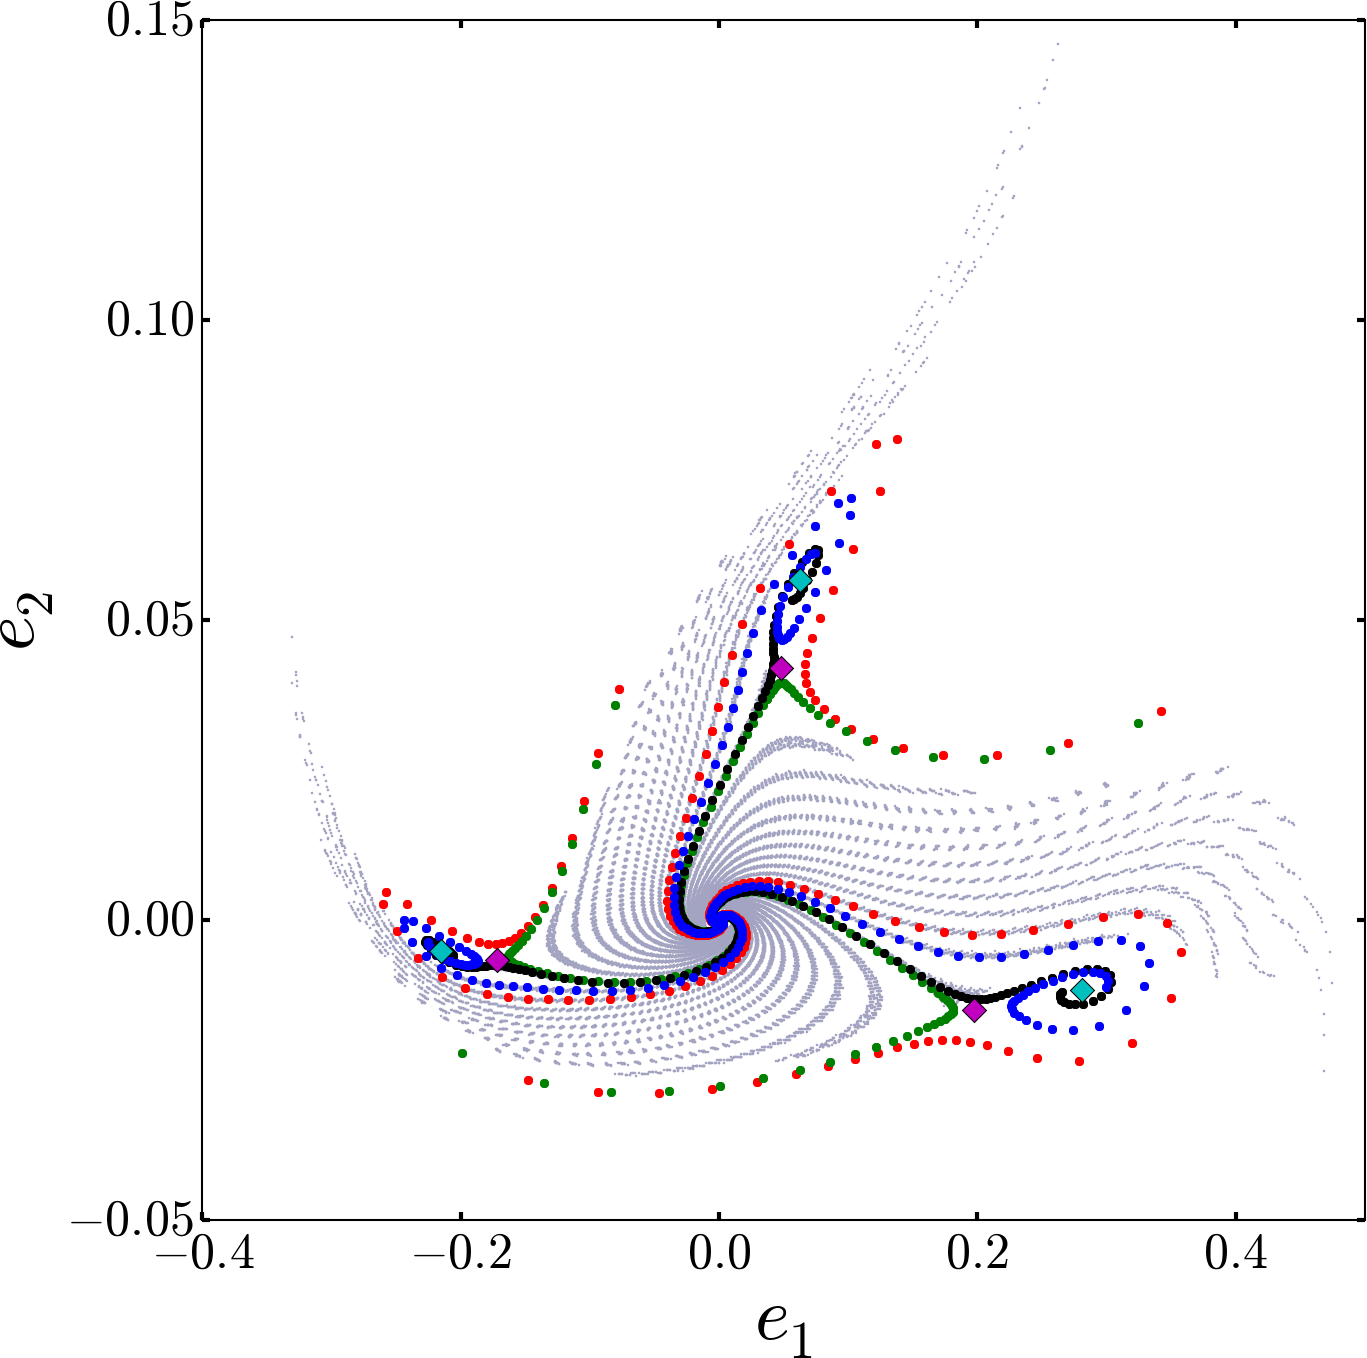
\includegraphics[height=0.45\textwidth]{UnstMan21p36png}
    (b) 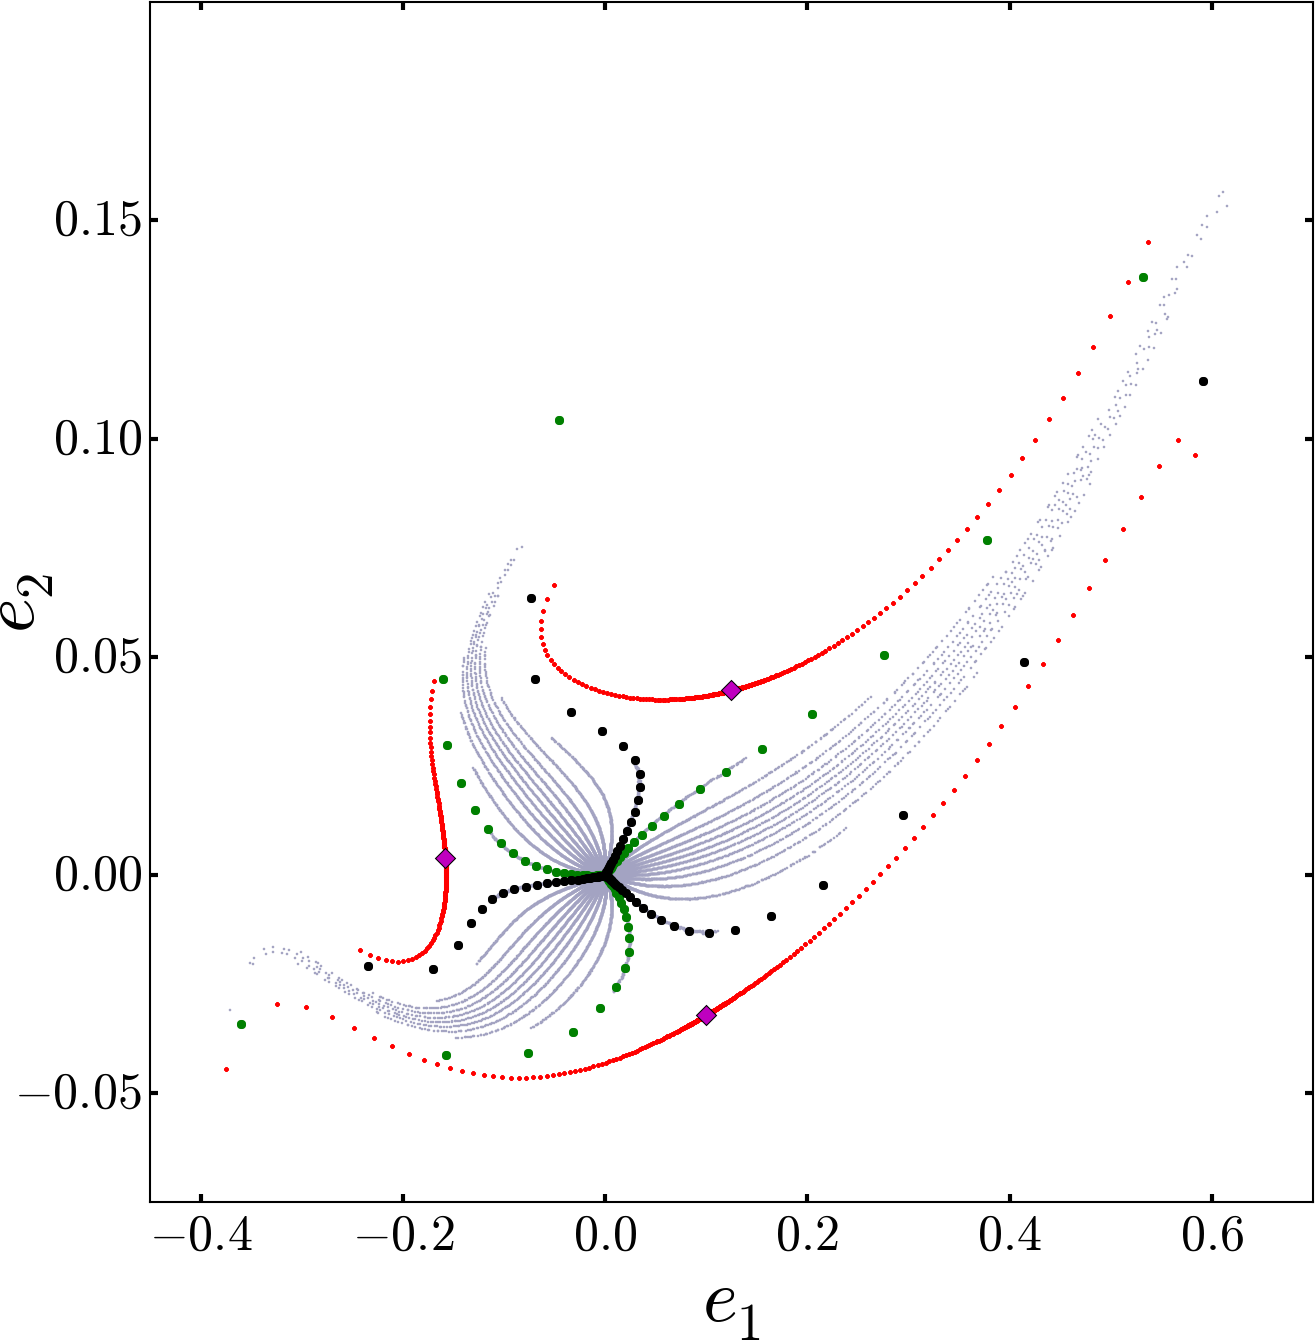
\includegraphics[height=0.45\textwidth]{UnstManPPO4L21p48png}
    \caption[Heteroclinic connections between \rpo s]{
        \label{f-Connections}
        (a) Unstable manifold (gray) of $p_{0}$ on the Poincar\'e
        section at $L=21.36$. Colored dots
        correspond to different individual trajectories within
        the unstable manifold with qualitatively different
        properties. Diamond shaped markers correspond to the
        period-3 orbits $p_{1}$ (magenta) and $p_{2}$ (cyan).
        (b) Unstable manifold of $p_{0}$ (gray) and two orbits
        (black and green) within at $L=21.48$. Red points lie on
        the one-dimensional unstable manifold of $p_{1}$.
    }
\end{figure}

\begin{quote}
    ``Strikingly similar structures of ergodic trajectories and periodic
orbits on the Poincar\'e section \reffig{f-Poincare} motivated us
to study unstable manifolds of the periodic orbits. However, we have not
succeeded in identifying one important \rpo\ (out of $479$!) whose
invariant manifolds form the shape of this attractor.
For this reason, we decided to first investigate the system by varying
its size and study its bifurcations, in order to see whether one of
these orbits plays the key role in shaping the strange attractor.''
\end{quote}

\begin{figure}[h]
    \centering
    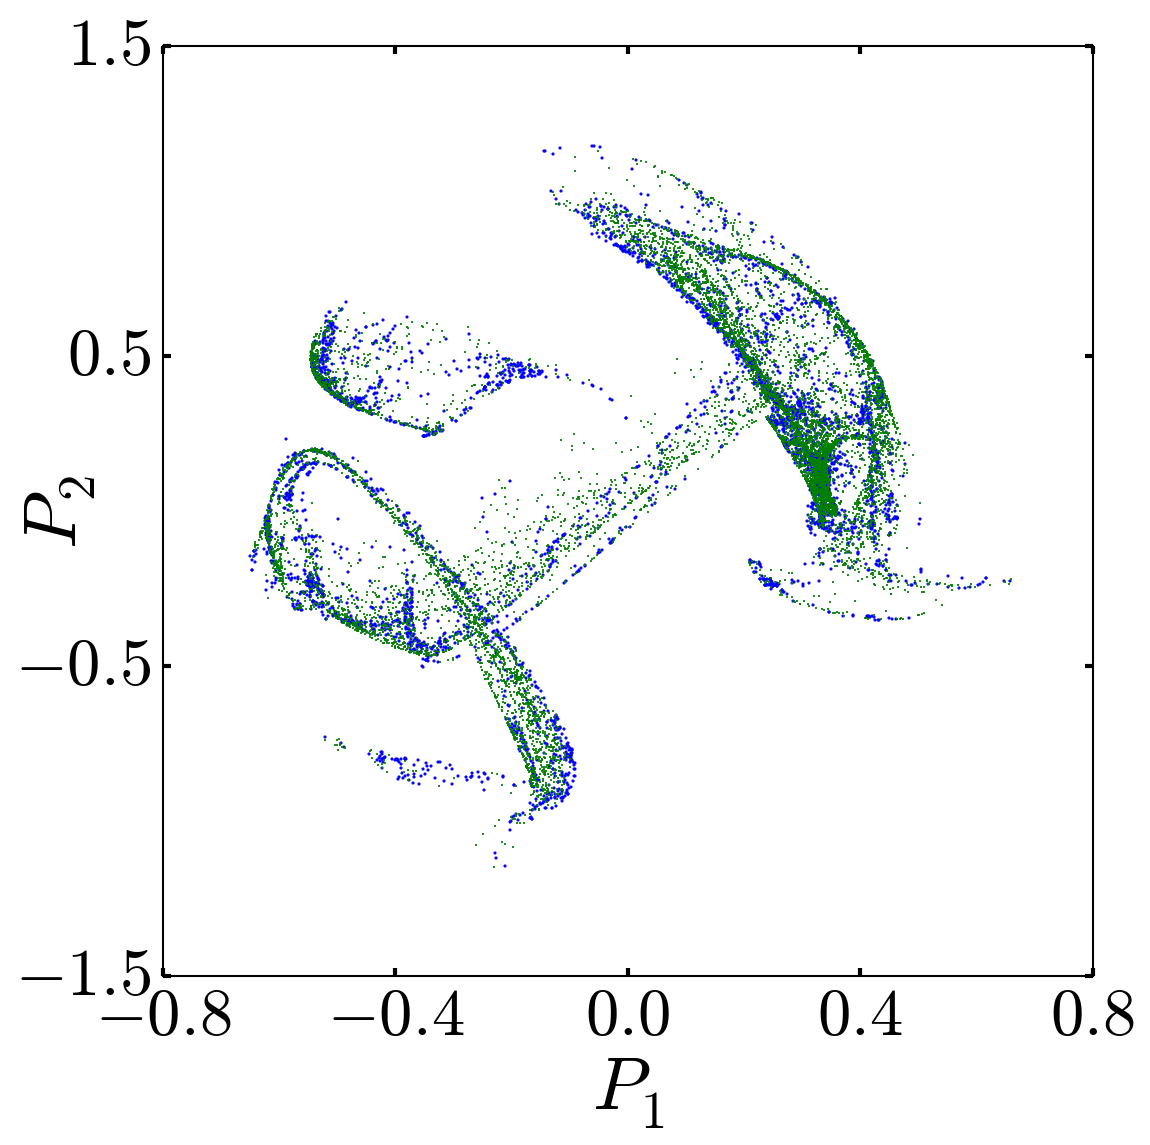
\includegraphics[width=0.65\textwidth]{ksPoincarethesis}
    \caption[A global Poincar\'e section for \KS\ system.]{
        Intersections of the long ergodic trajectory (green) and $479$
        \po s
        (blue) with the Poincar\'e section which contains the origin
        of the pca coordinates
        (empirical mean) and is parallel to
        $(P_1, P_2)$ plane.
    }
    \label{f-Poincare}
\end{figure}

Making sense of \reffig{f-Poincare}, the amazingly thin and structured
strange attractor embedded in the 30\dmn\ symmetry-reduced \statesp\
is ongoing research (promise to D. Barkley will be honored!), and for us the
method of \On{2}-symmetry reduction presented in the current submission
is the essential step.

We note in passing that for us the $\SOn{2}\times \On{2}$ symmetry
reduction remains an outstanding problem, and we are grateful for any
pointers on how to fully reduce it. The problem is illustrated here by
\reffig{fig:PCAplot} from \refref{WiShCv15}: with only \SOn{2} reduction,
`exact coherent structures' appear either in pairs, or are self-dual
under the remaining discrete $Z_{2}$  symmetry. This might not appear as
much to the handling editor, but it is a big deal when one is
constructing symbolic dynamics\rf{lanCvit07}. For example, if
$\On{2}$-invariant symbolic
dynamics requires 4 letters, the unreduced
\SOn{2}-invariant one will require $4^2=16$
letters, with much more unwieldy Poincar\'e return maps that are 15-modal
rather than 3-modal.

%%%%%%%%%%%%%%%%%%%%%%%%%%%%%%%%%%%%%%%%%%%%%%%%%%%%%%%%%%%%%%%%%%%%%%%
\setlength{\unitlength}{.48\textwidth}
% former ../figs/figPCAplot
\begin{figure}[h]
    \centering
    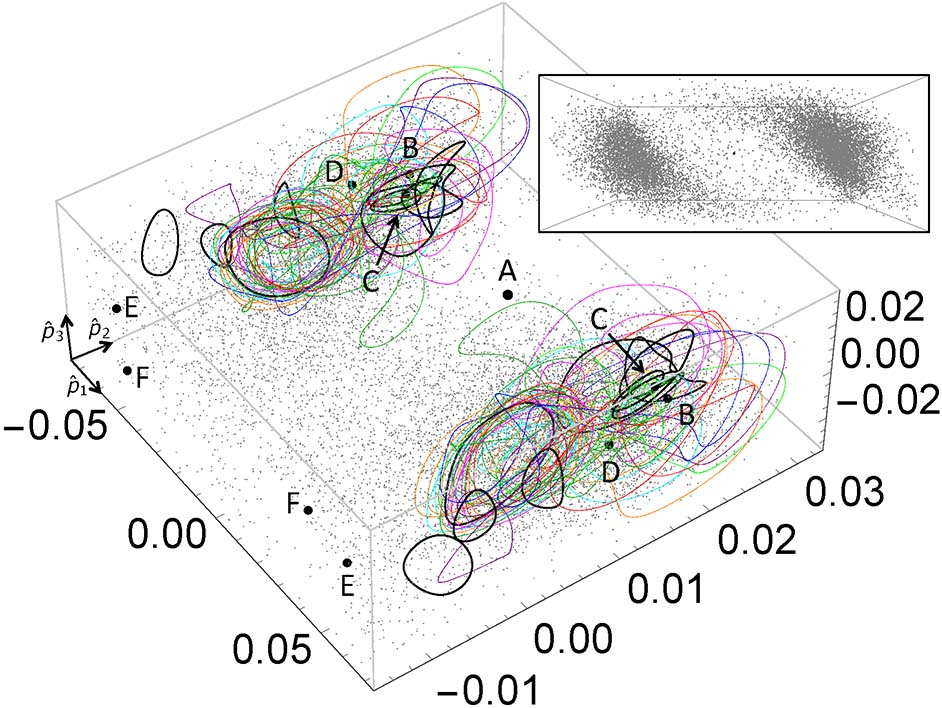
\includegraphics[width=\unitlength]{PREpca}
    \caption{ \label{fig:PCAplot}
            Projection of the symmetry-reduced infinite-dimensional {\statesp},
            together with the natural measure (the gray `cloud').
            32 \rpo s, together with \reqva\
            (A) $\TWRUN{N4U/3.28}{6482}$,
            (B) $\TWRUN{2.04}{8014}$,
            (C) $\TWRUN{2.03}{6494}$,
            (D) $\TWRUN{1.97}{6472}$,
            (E) $\TWRUN{1.98}{6491}$,
            (F) $\TWRUN{1.85}{6416}$.
            Due to a `rotate-and-reflect' symmetry,
            each solution appears twice, with the exception of (A)
            $\TWRUN{N4U/3.28}{6482}$ which
            belongs to the `rotate-and-reflect' invariant subspace. Our \rpo s capture
            the regions of high natural measure very well.
            The symmetry-invariant subspace has a
            strong repulsive influence, separating the natural measure into two
            weakly communicating regions.
    }
\end{figure}
%%%%%%%%%%%%%%%%%%%%%%%%%%%%%%%%%%%%%%%%%%%%%%%%%%%%%%%%%%%%%%%%%%%%%%%


We have gone into some detail here, as some of this motivational background
clearly needs to be included in the next revision of our manuscript.
Now to the paper at hand. In terms of editor input, there is not much to go on,
but we'll do our best.

\section{Responses to the editor}

\paragraph{(1) The handling editor helpfully notes:}

\begin{quote}
    ``The
authors do not cite standard references of equivariant bifurcation
theory and seem to be unaware of them. The methods of invariant
polynomials, which they use and call new, is a standard tool in
orbit space reduction, see e.g., the textbook \emph{Methods in
Equivariant Bifurcations and Dynamical Systems} by Pascal Chossat
and Reiner Lauterbach\rf{ChossLaut00}.''
\end{quote}

Were only the editor right, and we were ignorant of the literature,
%just a pair of lazy bums,
the life would have been so much easier. But we are diligent students of
Chossat and Lauterbach, and much more.  Every mathematician and
theoretical physicist has encountered symmetries in their research and is
fully confident that she knows how to use group theory when
needed\rf{PCgr}. Probably a  quarter of the GaTech Center for Nonlinear
Science library are books that deal with symmetries. Our main blog on the
subject is currently over 500 book pages, we have at least looked at and
at times studied in depth some 400 papers on symmetry reduction,
and in perhaps half of our weekly group meetings (3 different focus groups)
we discuss how to best deal with symmetries. As an
illustration of the literature we have studied, we append in
\refsect{sect:coment} a few excerpts of our commentary\rf{DasBuch} on the
subject -- we would be grateful for any expert comments on that.

So what is the problem?

The dynamical systems literature tends to
focus on \emph{local} problems: bifurcations of a single time-invariant
solution (\eqv, \reqv, \po\ or \rpo) in low-dimensional settings (3-5
coupled ODEs, 1\dmn\ PDE). The problem that we face is \emph{global}:
organizing and relating \emph{simultaneously} infinities of unstable \rpo
s in $\infty$\dmn\ \statesp s, orbits that are presumed to form the skeleton of
turbulence (see \refref{GibsonMovies} for a gentle introduction) and are
typically not solutions that possess the symmetries of the problem.
In this quest we found the standard equivariant bifurcation theory
literature not very helpful, as its general focus is on
bifurcations of solutions, which admit all or some of the symmetries
of the problem at hand.

We would be grateful if the handling editor could direct us to a
reference where $\On{2}$ invariant polynomials were computed using
``standard methods" for a state space dimension greater than --let's say-- 15.

We are certainly not aware of such a reference.  For high dimensions, standard
algorithms yields higher and higher order polynomials with increasing
number of syzygys. To the best of our knowledge, after 12+ dimensions,
computer algebra methods become completely impractical\rf{gatermannHab}.
In fact, the difficulty of computing invariant polynomials is clearly
stated in the reference suggested by the editor. Here is an excerpt
from Chossat and Lauterbach\rf{ChossLaut00}, Chapter 6, page 188:

\begin{quote}
``It should be emphasized here that these two reduction methods are
not equivalent, except in the simple example of bifurcation for the Hopf
normal form, and moreover they do not always work (the orbit space, in
particular, can be extremely difficult to compute).''
\end{quote}

As in war and love, everything is allowed in symmetry reduction, as long
as it serves the purposes of a particular application. The choice is
always a compromise between geometry (nonlinear coordinate redefintions,
nonlinear slice or `base' manifolds, motivated by the low-dimensional,
normal form intuition) and what is numerically feasible ( in
high-dimensional \statesp s, typically hyperplane slices). In our paper
this difficulty is overcome by implementing reflection-invariant
polynomials \emph{after} reducing \SOn{2} symmetry by \mslices.
In our invariant polynomials construction the polynomials are very
simple, the number of the polynomials is the same as the dimension of the
symmetry-reduced \statesp, no multinomial is of order higher than 2 so
the distortion of the \statesp\ in invariant coordinates is rather mild,
and there are \emph{no syzygies}, for any finite-\dmn\ truncation of the
Fourier basis.
Can the editor direct us to a reference that explains this ``standard
tool in orbit space reduction'' and thus show that there is nothing new
in our work? Or perhaps suggest a better method for the \On{2}
symmetry reduction, a method that scales well to 100\,000 dimensions?
We have studied
\refrefs{AGHO288,Choss93,Coma06,Dang86,Rodriguez1990,AshBoMe96,SmMoehHo05}
and much else, and have not found a better (or even feasible) method there.

Our introduction of polynomial invariants for an infinite sequence of
coordinates that change signs under reflection was inspired by
the invariant polynomials of ``the proto-Lorenz system'' of
\refrefs{GL-Mir93,GL-Gil07b}, which we cite in the paper. While we
did an extensive literature search (see our commentary,
\refsect{sect:coment}) for invariants like ours, we have
not found a similar construction for an infinite sequence of
coordinates. If the handling editor points us to a reference where a
similar approach is taken, or a method that would yield the
same result, we would be more than happy to cite it in the next revision.

Our paper introduces a new $\On{2}$-invariant symmetry-reduced
representation of any
$\On{2}$-equivariant PDE, without
any restriction on the truncation of the Fourier series. This
perhaps is of no interest if one only cares about bifurcations
in the small neighborhoods of invariant solutions, normal forms, etc.
However, as we explain in various places in the paper, our goal
is to understand the global organization of all numerically
exact time-invariant solutions (the infinity of \rpo s). That
requires tracking the global, curved unstable manifolds of
our numerically exact \rpo s. To this end, the bifurcation
sequence presented in the paper is simply an example of the
applicability of the our method in a high\dmn\ setting.
The heteroclinic connections of
relative periodic orbits as visualized in Poincar\'e maps of
\reffig{f-Connections} (figure~5 in the paper)
demonstrate our progress towards understanding what shapes the `turbulent' attractor
of \reffig{f-Poincare}. Again, we would be
happy to cite in our revised paper any
literature in which such objects were located for
PDEs in presence of both continuous and discrete symmetries.

\paragraph{(2) The handling editor concludes:}

\begin{quote}
``The paper might be interesting for other audiences who do not know
about equivariant bifurcation theory, but I do not think that the paper
is suitable for SIADS.''
\end{quote}

This is presumably either a statement about the style of presentation, or a
statement about the mission of SIADS.


Our submission is \emph{not}
a paper on equivariant bifurcations, it is a paper on global symmetry
reduction, and our intended audience are not the equivariant bifurcation
theory experts (though we believe they could profit from learning how
symmetry reduction works for global dynamics), but the broad group of
dynamical systems and numerical PDEs experts who need to apply symmetry
reduction to their specific modeling, fluid dynamics, \etc\ problems.
They represent a significant fraction of the SIAM members who contribute
to the biannual \emph{SIAM Conference on Dynamical Systems} PDEs, fluids
and dynamical systems sessions, a group traditionally allergic to
``gruppen-pest.'' Here is how our highly respected colleague Fabian
Waleffe feels about the matter:

\begin{quote}
How many Tylenols should I take with this?...
(never took group theory, still need to be convinced
that there is any use to this beyond mind-numbing formalizations.)
\end{quote}

It is this group of applied mathematicians that we have to reach, and we
try to make our presentation as simple and technical-jargon free as
possible (for example, the name ``Lie'' appears nowhere in our
fluid-dynamics papers on reduction of continuous symmetries, such as
\refref{ACHKW11}). The article is not written in the style of the classic
equivariant bifurcation theory papers, such as \refrefs{Field80,Krupa90},
because our intended readership would not read it if it were. And if we
were to cite every paper we found not helpful, the paper would be twice
as long and half as easy to navigate. Whether SIADS is to serve this
community is a decision for SIAM to make. Our current submission might
fall short of what we have hoped to communicate, but we would be grateful
for expert referees' technical suggestions as to how to bring it to that
level.

\bigskip
\bigskip
\bigskip

\noindent
Sincerely,
            \begin{quote}
            Nazmi Burak Budanur
            and
            Predrag Cvitanovi\'c \\
School of Physics\\
Georgia Institute of Technology\\
Atlanta, GA 30345-0430\\
\end{quote}




\newpage

\section{Commentary}
\label{sect:coment}

\remark{Literature.}{
We found Tinkham\rf{Tinkham} the most enjoyable as a
no-nonsense, the user friendliest introduction to the basic
concepts.
Slightly longer, but perhaps student-friendlier is
{\em Part I Basic Mathematics} of Dresselhaus~\etal\rf{Dresselhaus07}.
Byron and Fuller\rf{ByFu92}, the last chapter of volume two,
offers an introduction even more compact than Tinkham's.
For a summary of the theory of discrete groups see,
for example, \refref{stevenj}. Chapter 3 of Rebecca
Hoyle\rf{hoyll06} is a very student-friendly overview of
the group theory a nonlinear dynamicist might need, with
exception of the quotienting, reduction of dynamics to
a fundamental domain, which is not discussed at all.
We found
\HREF{en.wikipedia.org/wiki/Quotient_group}
{en.wikipedia.org/wiki/Quotient\_group} helpful.
Curiously,
we have not read any of the group theory books that Hoyle
recommends as background reading, which just confirms that
there are way too many group theory books out there. For
example, one that you will not find useful at all is
\refref{PCgr}. The reason is presumably that in the 20th
century physics (which motivated much of the work on the
modern group theory)
the focus is on the linear representations used in quantum
mechanics, crystallography and quantum field theory. We shall
need these techniques when we reduce the
linear action of evolution operators to irreducible
subspaces. However, here we are looking at nonlinear
dynamics, and the emphasis is on the symmetries of orbits,
their \reducedsp\ sisters, and the isotypic
decomposition of their linear stability matrices.

In ChaosBook we focus on chaotic dynamics, and skirt the theory of
bifurcations, the landscape between the boredom of regular
motions and the thrills of chaos.
Chapter 4 of Rebecca Hoyle\rf{hoyll06} is a
student-friendly introduction
to the treatment of bifurcations in presence of symmetries,
worked out in full detail and generality in monographs by
Golubitsky, Stewart and Schaeffer\rf{golubII},
Golubitsky and Stewart\rf{golubitsky2002sp} and
Chossat and Lauterbach\rf{ChossLaut00}.
Term `stabilizer' is used, for example,
 by Broer \etal\rf{BHLV03} to refer to a {\po}
with $Z_2$ symmetry; they say that the relative or pre-periodic
segment is in this case called a `short \po.' In
Efstathiou\rf{Efst05} a subgroup of
`short \po' symmetries is referred to as a
`nontrivial isotropy group or stabilizer.'
Chap.~8 of Govaerts\rf{Govaerts00} offers a review
of numerical methods that employ equivariance with respect to
compact, and mostly discrete groups.
    } %end\remark{Literature}{

\remark{Ideal is not real.}{\label{rem:IdealNotReal}
The literature on symmetries in dynamical systems is immense, most of it
deliriously unintelligible. Would it kill
them\rf{hoyll06,MarRat99,golubitsky2002sp,GL-Gil07b} to say `symmetry of
orbit $p$' instead of carrying on about `isotropies, quotients, factors,
normalizers, centralizers and stabilizers?'
Group action being `free, faithful, proper, regular?' Symmetry-reduced
\statesp\ being `orbitfold?'
For the dynamical systems applications at
hand we need only the basic Lie group facts, on the level of any standard
group theory textbook\rf{hamer}. We found Roger Penrose\rf{Penr04}
introduction to the subject both enjoyable and understandable.
Chapter 2. of
\refref{BlumanSDE89} offers a pedagogical introduction to Lie
groups of transformations, and Nakahara\rf{Naka90} to Lie
derivatives and brackets. The presentation given here is in
part based on Siminos thesis\rf{SiminosThesis} and
\refref{SiCvi10}. The reader is referred to the monographs of
Golubitsky and Stewart\rf{golubitsky2002sp},
Hoyle\rf{hoyll06}, Olver\rf{OlverInv}, Bredon\rf{Bredon72},
and Krupa\rf{Krupa90} for more depth and rigor than would be
wise to wade into here.
    } % \remark{Ideal is not real

\remark{A brief history of relativity,}{\label{rem:SSLieGr}
or,
`Desymmetrization and its discontents'
(after \HREF{http://en.wikipedia.org/wiki/Civilization_and_Its_Discontents}
{Civilization and its discontents};
continued from \refrem{rem:IdealNotReal}).

Relative equilibria and relative periodic solutions are related by
symmetry reduction to equilibria and periodic solutions of the reduced
dynamics. They appear in many physical applications, such as celestial
mechanics, molecular dynamics, motion of rigid bodies, nonlinear waves,
spiralling patterns, and fluid mechanics. A \reqv\ is a solution which
travels along an orbit of the symmetry group at constant speed; an
introduction to them is given, for example, in
Marsden\rf{Marsd92}. % in Chapter 4
According to Cushman, Bates\rf{CushBat97} and Yoder\rf{Yode88}, C.
Huygens\rf{Huyg1673} understood the \reqva\ of a spherical pendulum many
years before publishing them in 1673. A reduction of the translation
symmetry was obtained by Jacobi (for a modern, symplectic implementation,
see Laskar \etal\rf{MaRoLa02}).
In 1892 German sociologist
\HREF{http://alo.uibk.ac.at/webinterface/library/ALO-BOOK_V01?objid=12421&zoom=6}
{Vierkandt}\rf{Vierkandt1892} showed that on a symmetry-reduced space
(the constrained velocity phase space modulo the action of the group of
Euclidean motions of the plane) all orbits of the rolling disk system are
periodic\rf{BlMaZe05}.
   % \HREF{http://www.ams.org/notices/200503/fea-bloch.pdf}{Bloch \etal}
According to Chenciner\rf{Chenc05}, the
first attempt to find (relative) periodic solutions of the
$N$-body problem was the 1896 short note by
\Poincare\rf{Poinc1896}, in the context of the 3-body
problem. \Poincare\ named such solutions `relative'.
\Reqva\ of the $N$-body problem (known in this
context as the Lagrange points, stationary in the co-rotating
frame) are circular motions in the inertial frame, and {\rpo
s} correspond to quasiperiodic motions in the inertial frame.
For \rpo s in celestial mechanics see also
\refref{Broucke75}. A striking application of \rpo s has been
the discovery of ``choreographies" in the $N$-body problems%
\rf{CheMon00,CGMS02,McCordMontaldi}.

The modern story on equivariance and dynamical systems starts perhaps
with S. Smale\rf{Smale70I} and M. Field\rf{Field70}, and on bifurcations
in presence of symmetries with Ruelle\rf{ruell73}. Ruelle proves that the
\stabmat/\jacobianM\ evaluated at an \eqv/fixed point $\ssp \in \pS_G$
decomposes into linear \irrep s of \Group, and that
stable/unstable manifold continuations of its eigenvectors inherit their
symmetry properties, and shows that an \eqv\ can bifurcate to a
rotationally invariant periodic orbit (\ie, \reqv).

Gilmore and Lettelier monograph\rf{GL-Gil07b} offers a very clear,
detailed and user friendly discussion of symmetry reduction by means of
Hilbert polynomial bases (do not look for `Hilbert' in the index,
though).
Vladimirov, Toronov and Derbov\rf{VlToDe98} use an invariant polynomial
basis to study bounding manifolds of the symmetry reduced \cLf\ and its
homoclinic bifurcations.
There is no general strategy how to construct a Hilbert basis;
clever low-dimensional examples have been constructed case-by-case.
Our textbook example, with one obvious
syzygy, is also misleading - syzygies proliferate
rapidly with increase in dimensionality.
The
determination of a Hilbert basis appears computationally
prohibitive for \statesp\ dimensions larger than
ten\rf{gatermannHab,ChossLaut00}, and rewriting the equations
of motions in invariant polynomial bases appears impractical
for high-dimensional flows.
Thus, by 1920's the problem of rewriting equivariant
flows as invariant ones was solved by Hilbert and Weyl, but
at the cost of introducing largely arbitrary extra dimensions,
with the reduced flows on manifolds of lower
dimensions, constrained by sets of syzygies. Cartan
found this unsatisfactory, and in 1935 he introduced\rf{CartanMF}
the notion of a {\em \movframe}, a map from a manifold
to a Lie group, which seeks no invariant polynomial basis,
but instead rewrites the reduced $\pS/\Group$ flow
in terms of $d-N$ {\em fundamental invariants} defined by
a generalization of the \Poincare\ section, a slice that
cuts across all group orbits in some open neighborhood. Fels
and Olver view the method as an alternative to the Gr\"obner
bases methods for computing Hilbert polynomials, to compute
functionally independent fundamental invariant bases for
general group actions (with no explicit connection to
dynamics, differential equations or symmetry reduction).
`Fundamental' here means that they can be used to generate
all other invariants. Olver's monograph\rf{OlverInv} is
pedagogical, but does not describe the original Cartan's
method. Fels and Olver papers\rf{FelsOlver98,FelsOlver99} are
lengthy and technical. They refer to Cartan's method as
method of `\movframe s' and view it as a special and less
rigorous case of their `moving coframe' method. The name
`moving coframes' arises through the use of Maurer-Cartan
form which is a coframe on the Lie group $\Group$, \ie, they
form a pointwise basis for the cotangent space. In
\refrefs{SiminosThesis,SiCvi10} the invariant bases generated
by the \movframe\ method are used as a basis to project a
full \statesp\ trajectory to the slice (\ie, the
$\pS/\Group$ \reducedsp).

The basic idea of the `\mslices' is intuitive and
frequently reinvented, often under a different name; for example,
it is stated without attribution as the problem 1. of Sect.
6.2 of Arnol'd {\em Ordinary Differential
Equations}\rf{arnold92}. The factorization
is stated on p.~31 of Anosov and
Arnol'd\rf{AnAr88}, who note, without further elaboration,
that in the vicinity of a point which is not fixed by the
group one can reduce the order of a system of differential
equations by the dimension of the group.
\refRef{ArKoNe88} refers to symmetry reduction as `lowering the order'.
For the definition of `slice' see, for example,  Chossat
and Lauterbach\rf{ChossLaut00}. Briefly, a submanifold $\pS_{\slicep}$
containing $\slicep$ is called a {\em slice} through
$\slicep$ if it is invariant under isotropy
$\Group_{\slicep(\pS_{\slicep})}=\pS_{\slicep}$. If $\slicep$ is a
fixed point of $\Group$, than slice is invariant under the
whole group. The slice theorem is explained, for example, in
\HREF{http://eom.springer.de/S/s120150.htm} {Encyclopaedia of
Mathematics}.
Slices tend to be discussed in contexts much more difficult
than our application - symplectic groups, sections in absence
of global charts, non-compact Lie groups. We follow
\refref{rowley_reconstruction_2000} in referring to a local
group-orbit section as a `slice'. \refRefs{Bredon72,GuiSte90}
and others refer to global group-orbit sections as
`cross-sections', a term that we would rather avoid, as it
already has a different and well established meaning in
physics. Duistermaat and Kolk\rf{DuiKol00} refer to `slices',
% on p. 103,
but the usage goes back at least to Guillemin and
Sternberg\rf{GuiSte90} in 1984, Palais\rf{Pal61} in 1961 and
Mastow\rf{Mostow57} in 1957. Bredon\rf{Bredon72} discusses
both cross-sections and slices. Guillemin and
Sternberg\rf{GuiSte90} define the `cross-section', but
emphasize that finding it is very rare: ``existence of a
global section is a very stringent condition on a group
action. The notion of `slice' is weaker but has a much
broader range of existence.''

Several important fluid dynamics flows exhibit continuous symmetries
which are either $\SOn{2}$ or products of $\SOn{2}$ groups, each of which
act on different coordinates of the {\statesp}. The \KS\
equations\rf{KurTsu76,Siv},
{\pCf}\rf{Visw07b,GHCW07,HGC08,HalcrowThesis}, and
pipe flow\rf{Wk04,Kerswell05} all have continuous symmetries of this
form.
In the 1982 paper Rand\rf{Rand82} explains how
presence of continuous symmetries gives rise to rotating and
modulated rotating (quasiperiodic) waves in fluid dynamics.
Haller and Mezi\'c\rf{HaMe98} reduce symmetries of
three\dmn\ volume-preserving flows and reinvent
\mframes, under the name `orbit projection map'. There is
extensive literature on reduction of symplectic manifolds
with symmetry; Marsden and Weinstein 1974 article\rf{MaWe74}
is an important early reference. Then there are studies of
the reduced phase spaces for vortices moving on a sphere such
as \refref{Kirwan88}, and many, many others.

Reaction-diffusion systems are often equivariant with respect
to the action of a finite dimensional (not necessarily
compact) Lie group. Spiral wave formation in such nonlinear
excitable media was first observed in 1970 by Zaikin and
Zhabotinsky\rf{ZaZha70}. Winfree\rf{Winfree73,Winfree1980}
noted that spiral tips execute meandering motions. Barkley
and collaborators\rf{BaKnTu90,Barkley94} showed that the
noncompact Euclidean symmetry of this class of systems
precludes nonlinear entrainment of translational and
rotational drifts and that the interaction of the Hopf and
the Euclidean eigenmodes leads to observed quasiperiodic and
meandering behaviors. Fiedler, in the influential 1995 talk
at the Newton Institute, and Fiedler, Sandstede, Wulff,
Turaev and  Scheel\rf{FiSaScWu96,SaScWu97,SaScWu99a,FiTu98}
treat Euclidean symmetry bifurcations in the context of
spiral wave formation. The central idea is to utilize the
semidirect product structure of the Euclidean group $E(2)$ to
transform the flow into a `skew product' form, with a part
orthogonal to the group orbit, and the other part within it.
They refer to a linear slice
\pSRed\ near \reqv\ as a {\em Palais slice}, with Palais
coordinates.
As the choice of the slice is arbitrary, these
coordinates are not unique. According to these authors, the
skew product flow was first written down by
Mielke\rf{Mielke91}, in the context of buckling in the
elasticity theory. However, this decomposition is no doubt
much older. For example, it was  used by
Krupa\rf{Krupa90,ChossLaut00} in his local slice study of
bifurcations of \reqva. Biktashev, Holden, and
Nikolaev\rf{BiHoNi96} cite Anosov and Arnol'd\rf{AnAr88}  for
the `well-known' factorization and write
down the slice flow equations.

Neither Fiedler \etal\rf{FiSaScWu96} nor Biktashev
\etal\rf{BiHoNi96} implemented their methods numerically.
That was done by Rowley and Marsden for the
Kuramoto-Sivashinsky\rf{rowley_reconstruction_2000} and the
Burgers\rf{rowley_reduction_2003} equations, and Beyn and
Th\"ummler\rf{BeTh04,Thum05} for a number of
reaction-diffusion systems, described by parabolic partial
differential equations on unbounded domains. We recommend the
Barkley paper\rf{Barkley94} for a clear explanation of how
the Euclidean symmetry leads to spirals, and the Beyn and
Th\"ummler paper\rf{BeTh04} for inspirational concrete
examples of how `freezing'/\-`slicing' simplifies the
dynamics of rotational, traveling and spiraling \reqva.
Beyn and Th\"ummler write the solution as a composition of
the action of a time dependent group element $\LieEl(t)$ with
a `frozen', in-\slice\ solution $\hat{u}(t)$.
In their nomenclature, making a \reqv\
stationary by going to a \comovframe\ is `freezing' the
traveling wave, and the imposition of the phase condition
(\ie, \slice\ condition  is the `freezing
ansatz'.  They find it more convenient to make use of the
equi\-vari\-ance by extending the \statesp\ rather than reducing
it, by adding an additional parameter and a phase condition.
The `freezing ansatz'\rf{BeTh04} is identical to the Rowley
and Marsden\rf{rowley_reduction_2003} and our slicing, except
that `freezing' is formulated as an additional constraint,
just as when we compute periodic orbits of ODEs we add
Poincar\'e section as an additional constraint, \ie, increase
the dimensionality of the problem by 1 for every continuous
symmetry.

%    \ES{Is this {\csection} related to a cross-section in a
%    $\Group$-bundle? In other words, can we interpret the
%    latter as a submanifold in total space \pS\ of a
%    $\Group$-bundle $(\pS,\pi,\pS/\Group)$? }


 Several symmetry
reduction schemes are reviewed in \refref{SiCvi10}. Here we
describe the
\mslices\rf{rowley_reconstruction_2000,BeTh04,FrCv11}, the
only method that we find practical for a symmetry reduction of
chaotic solutions of highly nonlinear and possibly also high\dmn\ flows.
Our derivation follows most closely
Rowley and Marsden\rf{rowley_reduction_2003} who, in the
pattern recognition setting refer to the \slice\ point as a
`template', and refer to the `reconstruction
equation'\rf{Marsd92,MarsdRat94}. They also describe the `method
of connections' (called `orthogonality of time and group
orbit at successive times' in \refref{BeTh04}), for which the
reconstruction equation denominator is
$\braket{\groupTan(\sspRed)} {\groupTan(\sspRed)}$ and thus
non-vanishing as long as the action of the group is regular.
This avoids the spurious \slice\ singularities, but it is not
clear what the `method of connections' buys us otherwise. It
does not reduce the dimensionality of the \statesp, and it
accrues `geometric phases' which prevent \rpo s from closing
into \po s.
Geometric phase in laser equations, including \cLe,
has been studied in
\refref{ToDe94,ToDe94a,NiHa91,NiHa92,NiHa92a}.
Another theorist's temptation is to hope that a continuous
symmetry would lead us to a conserved quantity. However,
Noether theorem requires that equations of motion be cast in
Lagrangian form and that the Lagrangian exhibits variational
symmetries\rf{Bluman07,BlumanAnco02}. Such variational
symmetries are hard to find for dissipative systems.

In general relativity `symmetry reduction' is a method of finding exact
solutions by imposing symmetry conditions to obtain a reduced system of
equations, \ie, restricting the set of solutions considered to an
invariant subspace. This is not what we mean by `symmetry reduction'
in this monograph.

References to `cyclists'
are bit of a joke in more ways than one.
First, `cyclist',
`pedestrian' throughout ChaosBook.org refer jokingly both to
the title of Lipkin's {\em Lie groups for
pedestrians}\rf{Lipkin66} and to our preoccupations with
\HREF{http://www.cns.gatech.edu/~predrag/friends/Predrag/MidnightRider75/mrider.html}
     {actual cycling}. Lipkin's `pedestrian' is fluent in
Quantum Field Theory, but wobbly on Dynkin diagrams. More to the point,
it is impossible to dispose of Lie groups in a page of text.
As a antidote to the brevity of exposition here,
consider reading
Gilmore's monograph\rf{gilmore08} which offers a quirky, personal and
enjoyable distillation of a lifetime of pondering Lie groups. As seems to
be the case with any textbook on Lie groups, it will not help you with
the problem at hand, but it is the only place you can learn both what
Galois actually did when he invented the theory of finite groups in 1830,
and what, inspired by Galois, Lie actually did in his 1874 study of
symmetries of ODEs. Gilmore also explains many things that we pass over
in silence here, such as matrix groups, group manifolds, and compact
groups.

One would think that with all this literature the case is
shut and closed, but not so. Applied mathematicians are
inordinately fond of bifurcations, and almost all of the
previous work focuses on \eqva, \reqva, and their
bifurcations, and for these problems a single \slice\ works
well. Only when one tries to describe the totality of chaotic
orbits does the non-global nature of slices become a serious
nuisance.

%\authorESPC
    } % \remark{A brief history of relativity



\newpage
\printbibliography[title={References}
                  ] %, type=online]  % if not using default "Bibliography"

\end{document}
